\documentclass[10pt,aspectratio=169]{beamer}

\usetheme[progressbar=frametitle]{metropolis}

\usepackage{appendixnumberbeamer}
\usepackage{booktabs}
\usepackage[scale=2]{ccicons}

\usepackage[normalem]{ulem}
\usepackage{subcaption}
\usepackage{tikz}
\usepackage{minted}
\usepackage{pgfplots}
\usepgfplotslibrary{dateplot}
\usepackage{csquotes}
\usepackage{amssymb}
\usepackage{pifont}
\usepackage{xcolor}
\newcommand{\cmark}{\ding{51}}
\newcommand{\xmark}{\ding{55}}
\newcommand{\done}{\rlap{$\square$}{\raisebox{2pt}{\large\hspace{1pt}\textcolor{green}{\cmark}}}\hspace{-2.5pt}}
\newcommand{\wontfix}{\rlap{$\square$}{\large\hspace{1pt}\textcolor{red}{\xmark}}}
\newcommand{\partialdone}{\rlap{$\square$}{\raisebox{2pt}{\large\hspace{1pt}\textcolor{orange}{\cmark}}}\hspace{-2.5pt}}

% \usepackage[backend=biber, style=numeric, citestyle=ieee]{biblatex}
\usepackage[backend=biber, citestyle=authortitle, maxbibnames=99]{biblatex}
\renewcommand{\footnotesize}{\fontsize{6pt}{6pt}\selectfont}
\addbibresource{references_local.bib}

\usepackage{pgfpages}
% \setbeamertemplate{note page}{\vspace*{0.75cm}\insertnote}
% \setbeameroption{show notes on second screen=right}
\setbeameroption{show notes}
% \setbeameroption{hide notes}


\title{Assessing the Viability of Rust in HPC}
\subtitle{3\textsuperscript{rd} year project presentation}
\author{Edmund Goodman}
\date{\today}


% ================================ %

\begin{document}

\maketitle
    \note[itemize]{
        \item Agenda will be:
        \begin{enumerate}
            \item Project background
            \item Translation process
            \item Equivalence checking
            \item Performance analysis and demo
            \item Project management
            \item Conclusion
        \end{enumerate}
    }

% \begin{frame}{Agenda}
%   \setbeamertemplate{section in toc}[sections numbered]
%   \tableofcontents%[hideallsubsections]
% \end{frame}

\begin{frame}{Before we begin...}
\begin{itemize}
    \item The performance analysis section will analyse benchmark runs
    \vspace*{0.5cm}
    \item I'm going to use a tool I built to start some of on DCS batch compute
        % \note<2>{\texttt{ssh kudu}\newline}
        % \note<2>{\texttt{cd ~/Desktop/project/hpccg-rs/hpc-multibench}\newline}
        % \note<2>{\texttt{poetry run python3 -m hpc\_multibench -y yaml\_examples/kudu/strong\_weak\_scaling.yaml record}}
    \begin{itemize}
        \item \alert{We will come back and explore them later, once they have completed!}
    \end{itemize}
\end{itemize}
\end{frame}

\section{Project Background}

\begin{frame}{The Rust Language \ i}
    % \begin{tikzpicture}[remember picture,overlay]
    %     \node[xshift=-1.2cm,yshift=-1.8cm] at (current page.north east) {
\includegraphics[width=0.15\textwidth]{images/ferris.png}};
    % \end{tikzpicture}
    \begin{itemize}
        \item Originally developed by Mozilla, and released in 2010
            \note[item]{Relatively young language, 14 years to C++'s 45\newline}
        \item Its website claims \footcite{RustProgrammingLanguage} it is:
        \begin{itemize}
            \item Performant
                \note[item]{No garbarge collection needed}
                \note[item]{Offers low-level abstractions for the computer hardware, facilitating performant code\newline}
            \item Productive
                \note[item]{Robust toolchain, including canonical linters (\texttt{clippy}), auto-formatters (\texttt{rustfmt}), and a centralised package repository (\texttt{crates.io})\newline}
            \item Reliable
                \note[item]{Rich type system, with foundation in programming languages like Haskell}
                \note[item]{Guarantees of safety by preventing undefined behaviour at compile time\newline}
        \end{itemize}
        \vspace*{0.25cm}
        \item Eliminates ``undefined behaviour'' by compiler rules
            \note[item]{Specifically, its ownership model which works by counting mutable and immutable references to data}
        \begin{itemize}
            \item Encompasses memory and thread safety
            \item Over 70\% of security bugs in the Chromium project related to memory safety \footcite{MemorySafety} % serious security bugs
        \end{itemize}
        \vspace*{0.25cm}
        \item Voted ``most loved'' programming language in StackOverflow's developer survey \footcite{StackOverflowDeveloper}
        \vspace*{0.25cm}
    \end{itemize}
\end{frame}

\begin{frame}{The Rust Language \ ii}
    % \begin{tikzpicture}[remember picture,overlay]
    %     \node[xshift=-1.2cm,yshift=-1.8cm] at (current page.north east) {
\includegraphics[width=0.15\textwidth]{images/ferris.png}};
    % \end{tikzpicture}
    Has been in the news even in the last month due to:
    \begin{itemize}
        \item White House Office of the National Cyber Director publishing a press release ``Future Software Should Be Memory Safe'' \footcite{PressReleaseFuture2024}  % (February 26th)
            \note[item]{Explicitly mentioning moving critical codebases to Rust as a part of US national cyber security policy}
        \item Google pledging \$1 million to improve Rust/C++ interoperability \footcite{ImprovingInteroperabilityRust}  % (February 5th)
        \begin{itemize}
            \item<2-> \alert{Blog post mentions tooling such as \texttt{autocxx} as part of this effort}
                \note[item]{\texttt{autocxx}, is a tool to which I had already pull requested integration tests in the course of the project}
        \end{itemize}
    \end{itemize}

    \vspace{0.5cm}
    \only<3->{
        \begin{figure}[H]
            
\includegraphics[width=0.95\textwidth]{images/autocxx_pr.png}
            \caption{A screenshot of my merged pull request into \texttt{autocxx}}
            \label{fig:warwick_mantevo_link}
        \end{figure}
    }
\end{frame}

\begin{frame}{High-Performance Computing}
    \begin{displayquote}
        \vspace{0.2cm}
        ``Technology that uses clusters of powerful processors, working in \textbf{parallel}, to process massive multidimensional datasets (\textbf{big data}) and solve complex problems at \textbf{extremely high speeds}.'' -- IBM \footcite{WhatHPCIntroduction}
    \end{displayquote}
    % \vspace*{0.25cm}
    % \begin{itemize}
    %     \item Often referred to by the initialism ``HPC''
    %     \item Key characteristics from definition:
    %     \begin{itemize}
    %         \item Parallel computation
    %             \note[item]{Within UMA machines with vectorisation and threading}
    %             \note[item]{Across NUMA clusters over TCP/IP networks\newline}
    %         \item Large data-sets
    %         \item \alert{High speeds}
    %             \note[item]{Overall goal of HPC is going as fast as possible...}
    %     \end{itemize}
    % \end{itemize}
\end{frame}

\begin{frame}{Mantevo Suite}
    \begin{itemize}
        \item In the early 2010s, hardware limitations forced hardware/software co-design
        \item Pioneered the concept of mini-apps to facilitate this
        % \begin{itemize}
        %     % \item Small codebases for ease of use
        %     % \item Similar performance characteristics to larger applications
        %     % \item Facilitate co-design
        %     %     \note[item]{Easy predictors of full application performance, which can be deployed early in hardware development}
        %     \item Can be re-purposed to assess software instead of hardware
        % \end{itemize}
    \end{itemize}
    \vspace*{0.75cm}
    \begin{displayquote}
        \vspace{0.2cm}
        ``[Mini-apps are] \textbf{small} software programs whose \textbf{performance characteristics model full-scale applications}, yet require only \textbf{a fraction of the lines of code}, making [them] easier to study, design, and rewrite.'' -- Mantevo Suite summary \footcite{heroux2013mantevo}.
    \end{displayquote}
\end{frame}

\begin{frame}{Warwick's Link to the Mantevo Suite}
    \begin{figure}[H]
        
\includegraphics[width=0.35\textwidth]{images/warwick_mantevo_link.png}
        \caption{A screenshot of an appendix to the original Mantevo Suite paper, showing Stephen Jarvis' support for the project \footcite{heroux2013mantevo}.}
        \label{fig:warwick_mantevo_link}
    \end{figure}
        \note[item]{Perhaps this helps justify mini-apps as an interesting thing to think about?}
\end{frame}

\begin{frame}{High Performance Computing Conjugate Gradients (HPCCG) \ i}
    \begin{columns}[onlytextwidth]
        \column{0.5\textwidth}
            \begin{itemize}
                \item ``The original Mantevo mini-app'' \footcite{MantevoHPCCG2023}
                \vspace{0.5cm}
                \item Designed to be ``the best approximation to an unstructured implicit finite element or finite volume application in 800 lines or fewer.''
                \item Based on the iterative method of gradient descent for conjugate gradients first proposed by Hestnes and Steifel in 1952 \footcite{hestenesMethodsConjugateGradients1952}
                \item Small C++ codebase with dependent only on \texttt{OpenMP} and \texttt{MPI}
            \end{itemize}
        \column{0.5\textwidth}
            \begin{figure}[H]
                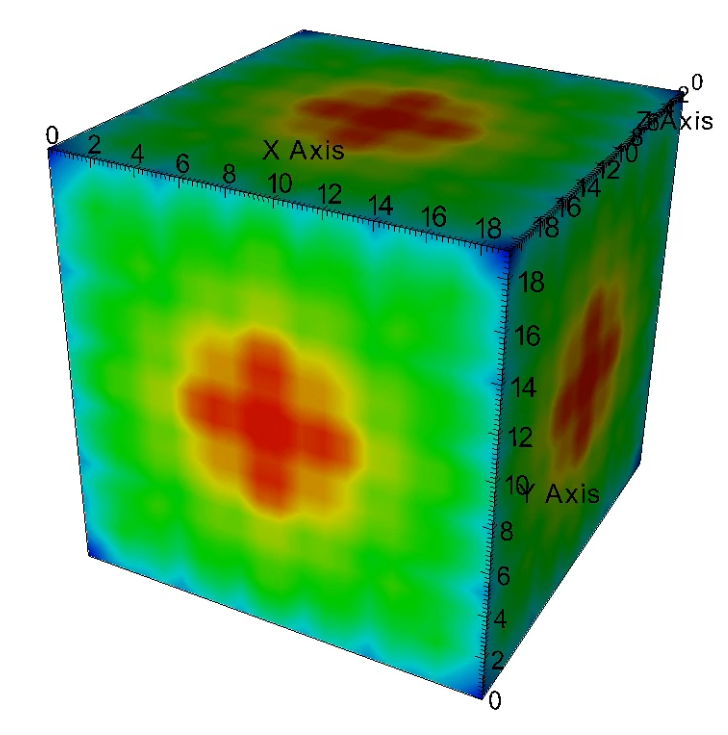
\includegraphics[width=0.75\textwidth]{images/acacgs_silo_output.png}
                \captionsetup{width=.9\linewidth}
                \caption{A screenshot of a silo visualisation from ACACGS, a C translation of HPCCG by Richard Kirk used in the CS257 coursework.}
                \label{fig:warwick_mantevo_link}
            \end{figure}
    \end{columns}
\end{frame}

\begin{frame}{High Performance Computing Conjugate Gradients (HPCCG) \ ii}
    % TODO: Regenerate images with terminal background set to #fafafa
    \begin{figure}
        \begin{subfigure}[c]{.45\textwidth}\centering
            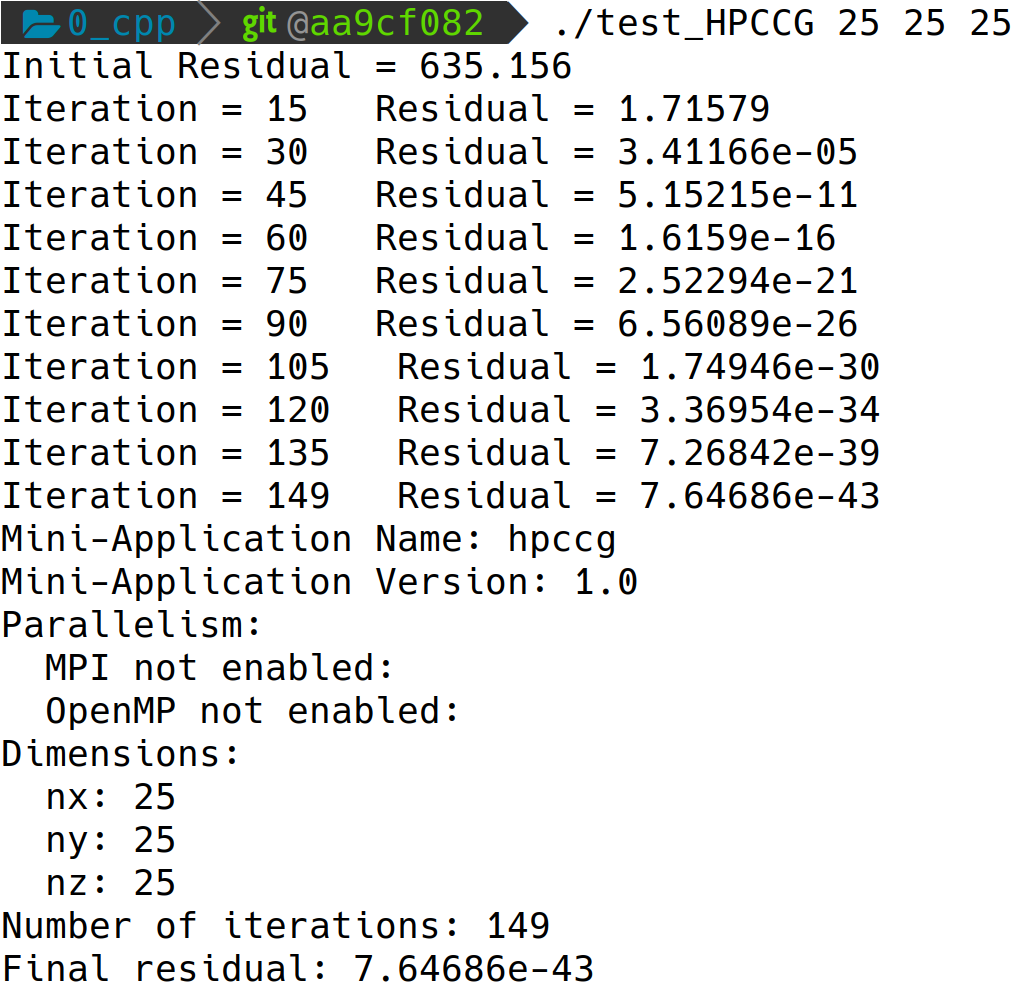
\includegraphics[width=0.95\textwidth]{images/hpccg-run.png}
            \label{fig:hpccg-run}
        \end{subfigure}%
        \begin{subfigure}[c]{.45\textwidth}\centering
            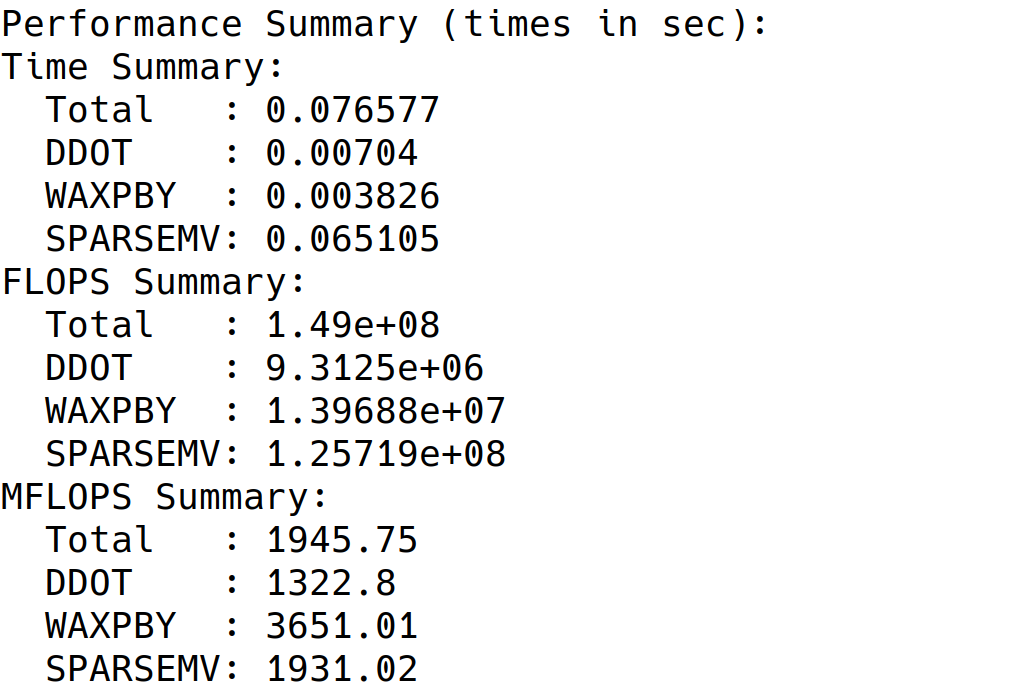
\includegraphics[width=0.95\textwidth]{images/hpccg-perf.png}
            \label{fig:hpccg-perf}
        \end{subfigure}
        \caption{The output from running HPCCG over a small mesh}
    \end{figure}
        \note[item]{HPCCG compiles to a standalone binary}
        \note[item]{Can be optionally compiled with OpenMP and MPI}
        \note[item]{This binary takes three parameters, the x y and z sizes of the mesh it runs on}
        \note[item]{It prints out its state as it performs iterations}
        \note[item]{When its done, it gives a performance summary}
\end{frame}

\begin{frame}{P$^3$HPC - not just performance!}
    % TODO: Re-work this slide? Add some images or something?
    % https://tex.stackexchange.com/questions/10060/how-to-draw-kiviat-diagrams for C++/Rust
    % Or an iron triangle breakdown

    % \begin{itemize}
    %     % \item <2-> Performance
    %     \item \alert<2>{Performance}
    %         \note[item]{This is something the project assesses!}
    %         \note[item]{Rust needs to nearly or as fast as C++ to be viable\newline}
    %     \vspace*{1cm}
    %     % \item <3-> Productivity
    %     \item \alert<3>{Productivity}
    %         \note[item]{Ergonomic syntax, most loved language with rich type system etc.}
    %         \note[item]{Good, canonical toolchain (\texttt{cargo}, \texttt{rustfmt}, \texttt{clippy}, ...)}
    %         \note[item]{Compiler check which make writing bug-free code easier\newline}
    %     \vspace*{1cm}
    %     % \item <4-> Portability
    %     \item \alert<4>{Portability}
    %         \note[item]{Rust toolchain is very portable (\texttt{rustc} / \texttt{LLVM} vs \texttt{gcc}, \texttt{icpc}, \texttt{clang}, ...)} % not like c++ with 5+ different proprietary compilers with slightly different flags
    %         \note[item]{Still capable of machine-specific optimisations with native architecture flag}
    % \end{itemize}
    
    \begin{figure}[H]
        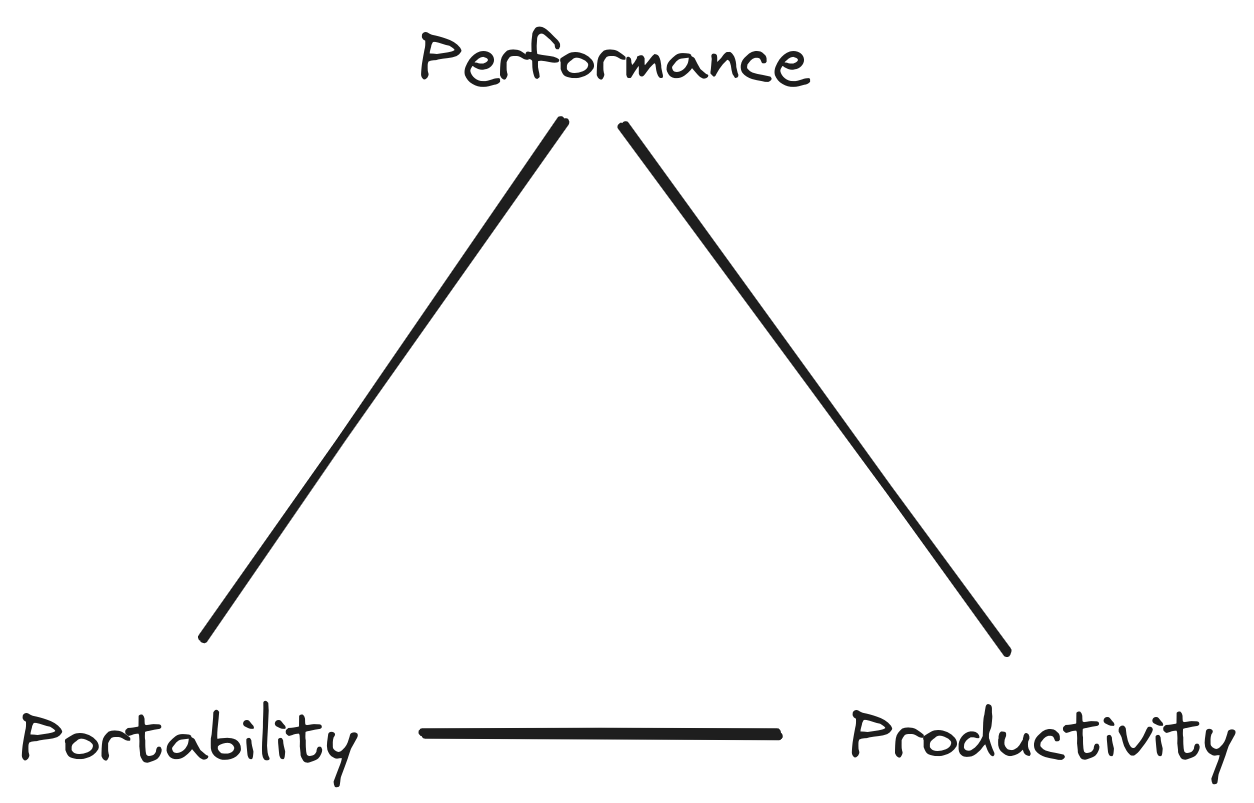
\includegraphics[width=0.5\textwidth]{images/excalidraw_p3_triangle.png}
        \vspace*{0.75cm}
        \label{fig:warwick_mantevo_link}
        % \caption{A diagram of three important aspects of high-performance software.}
    \end{figure}
    % \textbf{Why might Rust be a good fit for HPC?}
\end{frame}

% \begin{frame}{Existing work}
%     \begin{itemize}
%         \item Previous publications tend to address only performance
%         \item HPC is not only about performance
%         \item \alert{Aim to provide a holistic view of Rust's viability for HPC}
%     \end{itemize}
% \end{frame}

\begin{frame}{Project Initiation Requirements}
    \begin{itemize}
        \item[\done\ \ 1.]
          Select a target mini-app from ECP proxy applications or UK-MAC
          (\textbf{Must have})
        \item[\done\ \ 2.]
          Fuzz test the possible mini-apps for memory safety issues using static analysis tooling \footcite{stepanovMemorySanitizerFastDetector2015}
          (\textbf{Should have}, \textit{depends on 1})
    \end{itemize}
\end{frame}
    






\section{Translation Process}

\begin{frame}{C++ vs Rust}
    \begin{columns}[onlytextwidth]
        \centering
        \column{0.5\textwidth}
            \begin{itemize}
                \item There are more valid C++ programs\newline than (safe) Rust programs!
                    \note[item]{In a similar sense to moving from un-typed to type lambda calculi}
                    \note[item]{Could be considered an extension to Barendregt’s Lambda cube}
                \item Rust explicitly prohibits undefined behaviour by default
                \begin{itemize}
                    \item This is normally a good thing!
                \end{itemize}
                \item Translation is less trivial
                \begin{itemize}
                    \item Direct mapping might not exist
                    \item Can resort to \mintinline{rust}{unsafe} % TODO check other texttt tags
                \end{itemize}
            \end{itemize}
        \column{0.5\textwidth}
            \begin{figure}[H]
                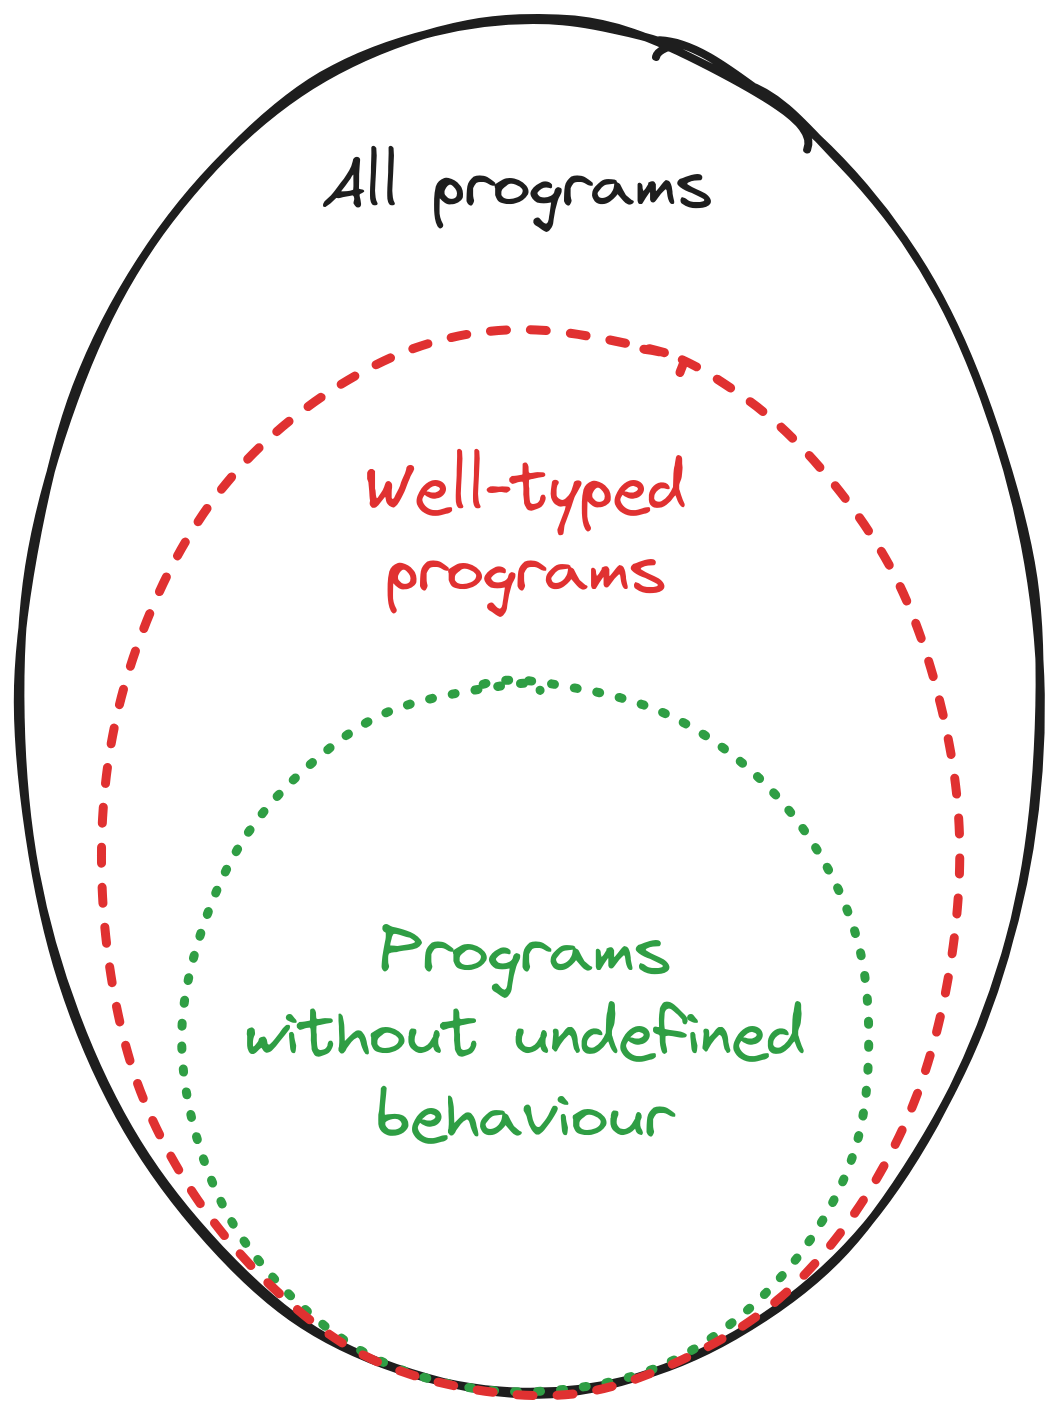
\includegraphics[width=0.65\textwidth]{images/excalidraw_programs_venn.png}
                % \captionsetup{width=.9\linewidth}
                \caption{A diagram to show the relative powers of increasingly restrictive program models.}
            \label{fig:warwick_mantevo_link}
        \end{figure}
    \end{columns}
    % The program model is different
    % The domain of valid C++ programs is a strict superset of Rust programs
    % This is helpful, as it means you can't write programs with undefined behaviour
    % This makes translation more difficult
\end{frame}

% \begin{frame}{Writing Performant Rust}
%     % TODO: Drop this slide
%     % There are a number of tricks you can do to make Rust more performant
%     % Many are enumerated in the Rust Performance Book
% \end{frame}

\begin{frame}[fragile]{Fearless Parallelism in Rust}
    \begin{itemize}
        \item One of Rust's key selling points is ``Fearless Parallelism''
        \begin{itemize}
            \item Many concurrency bugs moved from runtime to compile-time
                \note[item]{Ownership and type systems provide strong guarantees against undefined behaviour}
                \note[item]{Non thread-safe code often doesn't even compile, reducing the need to debug flaky race conditions}
            \item Ubiquitous crates provide very high-level abstractions
        \end{itemize}
    \end{itemize}    
    \vspace*{0.15cm}

    \begin{figure}
        \begin{subfigure}[c]{.55\textwidth}\centering
            \begin{minted}[escapeinside=||,linenos]{c++}
double dot_product (
    int n, double* x, double* y
) {
    double result = 0.0;
    for (int i = 0; i < n; i++) {
        result += x[i] * y[i];
    }
    return result;
}
            \end{minted}
            \label{fig:cpp-ddot-serial}
            \caption{C++ parallel implementation}
        \end{subfigure}%
        \begin{subfigure}[c]{.45\textwidth}\centering
            \begin{minted}[escapeinside=||,linenos]{rust}
pub fn dot_product(
lhs: &[f64], rhs: &[f64]
) -> f64 {
lhs.iter()
    .zip(rhs.iter())
    .map(|(x, y)| x * y)
    .sum()
}
            \end{minted}
            \label{fig:rust-ddot-serial}
            \vspace*{0.5cm}
            \caption{Rust serial implementation}
        \end{subfigure}
    \end{figure}
\end{frame}

\begin{frame}[fragile, noframenumbering]{Fearless Parallelism in Rust}
    \begin{itemize}
        \item One of Rust's key selling points is ``Fearless Parallelism''
        \begin{itemize}
            \item Many concurrency bugs moved from runtime to compile-time
                \note[item]{Ownership and type systems provide strong guarantees against undefined behaviour}
                \note[item]{Non thread-safe code often doesn't even compile, reducing the need to debug flaky race conditions}
            \item Ubiquitous crates provide very high-level abstractions
        \end{itemize}
    \end{itemize}    
    \vspace*{0.15cm}

    \begin{figure}
        \begin{subfigure}[c]{.55\textwidth}\centering
            \begin{minted}[escapeinside=||,linenos]{c++}
double dot_product (
    int n, double* x, double* y
) {
    double result = 0.0;
    #pragma omp parallel for
    for (int i = 0; i < n; i++) {
        result += x[i] * y[i];
    }
    return result;
}
            \end{minted}
            \label{fig:cpp-ddot-openmp-race}
            \caption{C++ parallel implementation}
            \only<2> {
                \begin{tikzpicture}[remember picture,overlay]
                    \draw[red, very thick] (-2.4,3.1) rectangle node[below, xshift=2.8cm, yshift=-0.3cm] {\huge{Data race!}} (-0.5,2.65);
                \end{tikzpicture}
            }
        \end{subfigure}%
        \begin{subfigure}[c]{.45\textwidth}\centering
            \begin{minted}[escapeinside=||,linenos]{rust}
pub fn dot_product(
lhs: &[f64], rhs: &[f64]
) -> f64 {
lhs.iter()
    .zip(rhs.iter())
    .map(|(x, y)| x * y)
    .sum()
}
            \end{minted}
            \label{fig:rust-ddot-serial-2}
            \vspace*{0.5cm}
            \caption{Rust serial implementation}
        \end{subfigure}
    \end{figure}
\end{frame}

\begin{frame}[fragile, noframenumbering]{Fearless Parallelism in Rust}
    \begin{itemize}
        \item One of Rust's key selling points is ``Fearless Parallelism''
        \begin{itemize}
            \item Many concurrency bugs moved from runtime to compile-time
                \note[item]{Ownership and type systems provide strong guarantees against undefined behaviour}
                \note[item]{Non thread-safe code often doesn't even compile, reducing the need to debug flaky race conditions}
            \item Ubiquitous crates provide very high-level abstractions
        \end{itemize}
    \end{itemize}    
    \vspace*{0.15cm}

    \begin{figure}
        \begin{subfigure}[c]{.55\textwidth}\centering
            \begin{minted}[escapeinside=||,linenos,breaklines]{c++}
double dot_product (
    int n, double* x, double* y
) {
    double result = 0.0;
#pragma omp parallel for reduction(+:result)
    for (int i = 0; i < n; i++) {
        result += x[i] * y[i];
    }
    return result;
}
            \end{minted}
            \label{fig:cpp-ddot-openmp-reduction}
            \vspace*{-0.5cm}
            \caption{C++ fixed parallel implementation}
        \end{subfigure}%
        \begin{subfigure}[c]{.45\textwidth}\centering
            \begin{minted}[escapeinside=||,linenos]{rust}
pub fn dot_product(
lhs: &[f64], rhs: &[f64]
) -> f64 {
lhs.iter()
    .zip(rhs.iter())
    .map(|(x, y)| x * y)
    .sum()
}
            \end{minted}
            \label{fig:rust-ddot-serial-3}
            \vspace*{1.15cm}
            \caption{Rust serial implementation}
        \end{subfigure}
    \end{figure}
\end{frame}

\begin{frame}[fragile, noframenumbering]{Fearless Parallelism in Rust}
    \begin{itemize}
        \item One of Rust's key selling points is ``Fearless Parallelism''
        \begin{itemize}
            \item Many concurrency bugs moved from runtime to compile-time
                \note[item]{Ownership and type systems provide strong guarantees against undefined behaviour}
                \note[item]{Non thread-safe code often doesn't even compile, reducing the need to debug flaky race conditions}
            \item Ubiquitous crates provide very high-level abstractions
        \end{itemize}
    \end{itemize}    
    \vspace*{0.15cm}

    \begin{figure}
        \begin{subfigure}[c]{.55\textwidth}\centering
            \begin{minted}[escapeinside=||,linenos,breaklines]{c++}
double dot_product (
    int n, double* x, double* y
) {
    double result = 0.0;
#pragma omp parallel for reduction(+:result)
    for (int i = 0; i < n; i++) {
        result += x[i] * y[i];
    }
    return result;
}
            \end{minted}
            \label{fig:cpp-ddot-openmp-reduction-2}
            \vspace*{-0.5cm}
            \caption{C++ fixed parallel implementation}
        \end{subfigure}%
        \begin{subfigure}[c]{.45\textwidth}\centering
            \begin{minted}[escapeinside=||,linenos]{rust}
use rayon::prelude::*; 

pub fn dot_product(
lhs: &[f64], rhs: &[f64]
) -> f64 {
lhs.par_iter()
    .zip(rhs.par_iter())
    .map(|(x, y)| x * y)
    .sum()
}
            \end{minted}
            \label{fig:rust-ddot-rayon}
            \caption{Rust Rayon implementation}
            \only<2> {
                \begin{tikzpicture}[remember picture,overlay]
                    \draw[red, very thick] (-0.9,3.1) rectangle (1.1,2.65);
                    \draw[red, very thick] (-2.6,3.6) rectangle (-0.5,3.15);
                    % \draw[red, very thick] (-2.5,3.75) rectangle (0,3.15);
                \end{tikzpicture}
            }
        \end{subfigure}
    \end{figure}
\end{frame}



\begin{frame}[fragile]{Clustered Computing in Rust}
    \begin{itemize}
        \item The Message Passing Interface (\texttt{MPI}) is a common way to distribute work across machines in a HPC computer cluster
        \item \texttt{MPI} has native C++ and FORTRAN implementations of its standard specification
        \item The \texttt{mpi} crate provides bindings from Rust into the C++ implementation
        % \begin{itemize}
        %     \item These bindings are designed to be ``rustic''
        %     \item They (so far\footnote{I am looking at pull requesting simple examples based on the integration tests}) have quite poor documentation
        % \end{itemize}
        % MPI spec
    \end{itemize}
    \vspace*{0.1cm}
    \begin{figure}
        \begin{subfigure}[c]{.5\textwidth}\centering
            \begin{minted}[linenos,breaklines]{c++}
#include <mpi.h>
MPI_Init(&argc, &argv);

MPI_Allreduce(
    &local_result, &global_result,
    1, MPI_DOUBLE, MPI_SUM,
    MPI_COMM_WORLD
);
            \end{minted}
            \label{fig:cpp-mpi}
            \vspace*{0.15cm}
            \caption{C++ MPI example}
        \end{subfigure}%
        \begin{subfigure}[c]{.5\textwidth}\centering
            \begin{minted}[linenos]{rust}
use mpi::collective::SystemOperation;
use mpi::traits::*;
let universe = mpi::initialize().unwrap();
let world = universe.world();

world.all_reduce_into(
    &local_result, &mut global_result,
    SystemOperation::sum()
);
            \end{minted}
            \label{fig:rust-mpi}
            \caption{Rust MPI example}
        \end{subfigure}
    \end{figure}
\end{frame}

\begin{frame}{Translation Requirements}
    \begin{itemize}
        \item[\done\ \ 5.]
          Write direct translation of serial version mini-app from C++ to Rust
          (\textbf{Must have}, \textit{depends on 1})
        \item[\done\ \ 6.]
          Modify serial version of translated code to be idiomatic Rust \footcite{endlerMreIdiomaticrust2023} 
          (\textbf{Should have}, \textit{depends on 5})
        \item[\done\ 11.]
          Modify the serial translated code to allow parallel execution
          (\textbf{Must have}, \textit{depends on 5})
        \item[\done\ 15.]
          Modify the parallel translated code to allow execution across clustered compute resources
          (\textbf{Could have}, \textit{depends on 11})
    \end{itemize}
    % TODO: Add lines of code written count here...
\end{frame}




\section{Equivalence Checking}

\begin{frame}{Equivalence Checking Techniques}
    % TODO: Add diagram showing rigour vs approach/ease for each methodology?
    \begin{itemize}
        \item Equivalence checking is critical to make performance comparisons fair
        \vspace*{0.5cm}
        \item Four different techniques considered
        \begin{enumerate}
            \item \alert<2>{End-to-end testing}
            % \begin{itemize}
            %     \item Run the program and examine its output
            %     \item Fairly effective for chaotic systems (like HPCCG), but can miss edge-cases in complex logic % Elucidated weird bug in both versions given non-associativity of floating point operations
            % \end{itemize}
            \item Formal methods
            % \begin{itemize}
            %     \item Techniques such as Hoare Logic \footcite{hoareAxiomaticBasisComputer1969} allow formal reasoning about programs
            % \end{itemize}
            \item LLVM analysis
            % \begin{itemize}
            %     \item Since the translated code does the same thing, generated LLVM IR may look similar
            % \end{itemize}
            \item \alert<2>{Unit testing}
            % \begin{itemize}
            %     \item Drive small code units and examine their outputs
            %     \item Can provide confidence about these units \textit{individually}
            %     \item Requires manual duplication across both languages, if no tooling exists...
            % \end{itemize}
        \end{enumerate}
    \end{itemize}
    % End-to-end testing (is fairly effective for chaotic systems like HPCCG)
    %  - Elucidated weird bug in both versions given non-associativity of floating point operations
    % Unit testing
    % Formal methods (refer to Hoare logic with neat example? conclusion as not too helpful)
    % LLVM analysis (just compare some clang decompiled code? conclusion as could be helpful, but high effort to build such a tool)
\end{frame}

\begin{frame}{Unit Tests with Test-Driven Development}
    \begin{figure}[H]
        \hspace*{-1cm}
        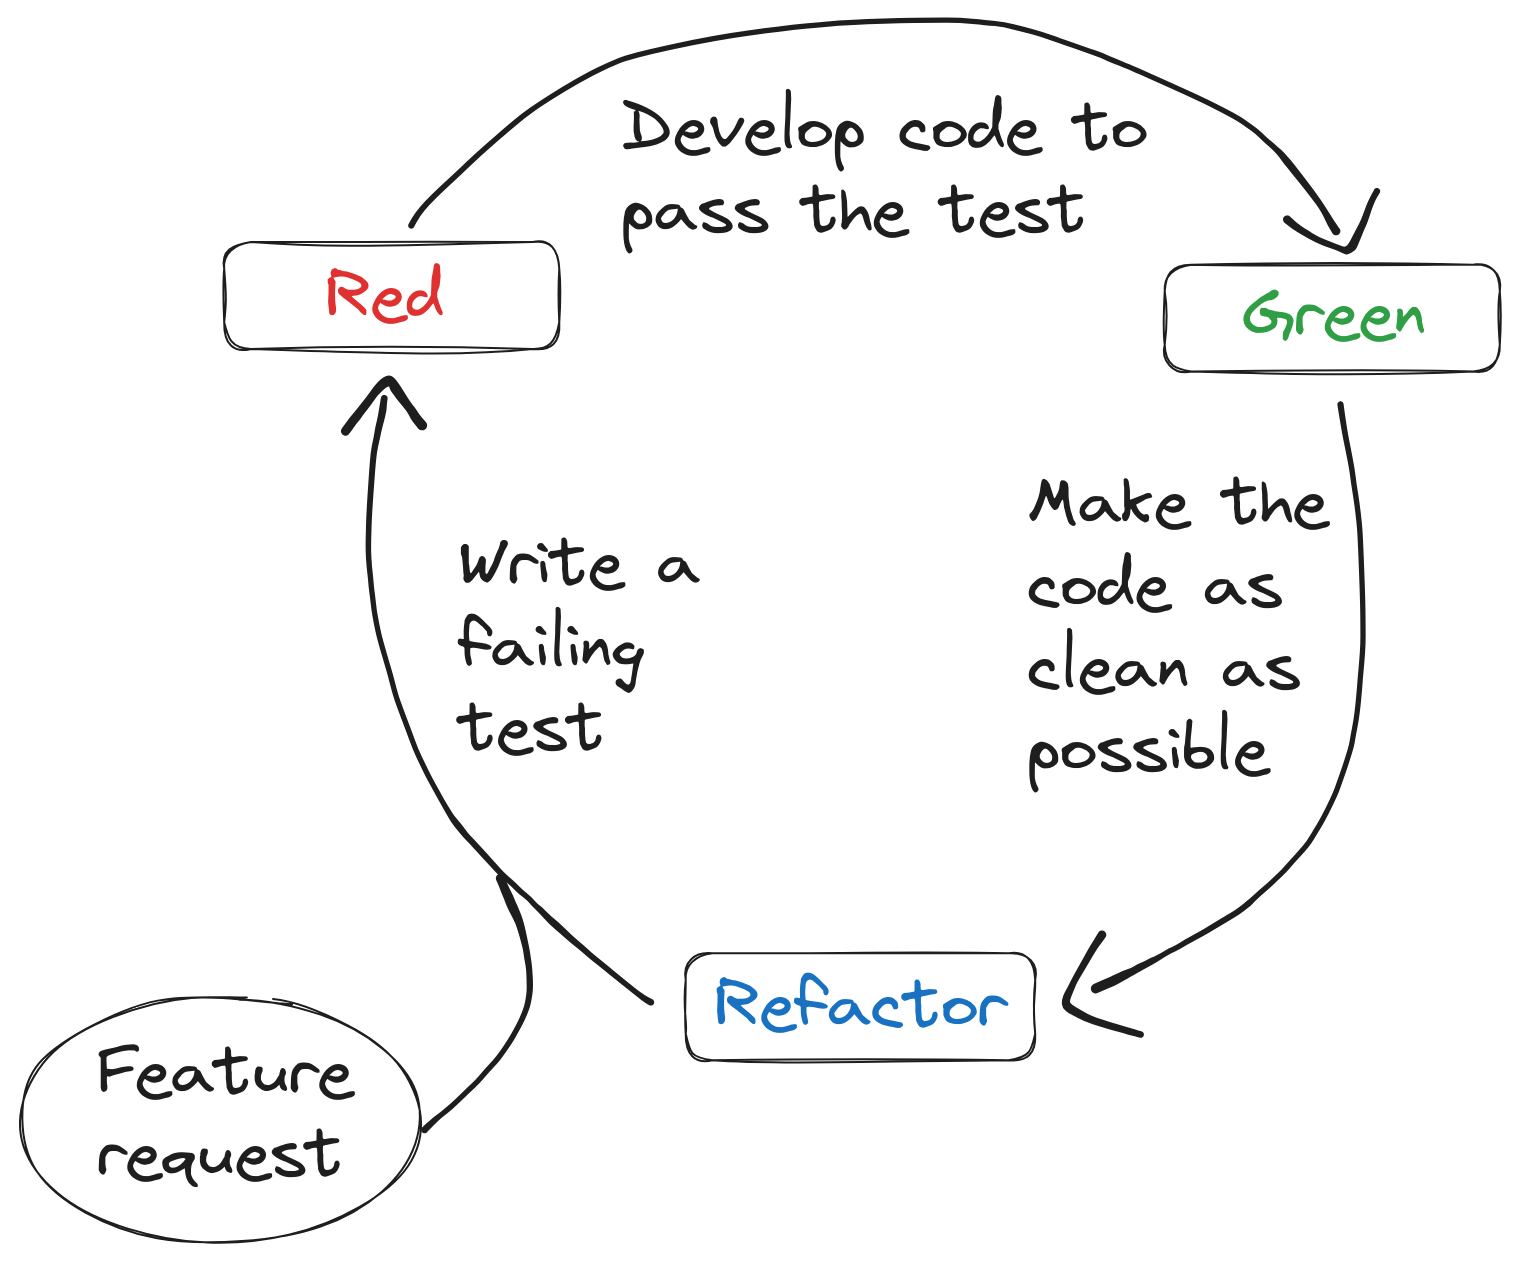
\includegraphics[width=0.45\textwidth]{images/excalidraw_tdd.png}
        \caption{A diagram showing the top-level workflow of the Test-Driven Development\footcite{beckTestDrivenDevelopment2022} methodology.}
        \label{fig:tdd_workflow}
    \end{figure}
    \only<2>{
        \vspace*{-0.5cm}
        \centering\large\alert{What if we could leverage this during translation...?}
        \vspace*{-0.4cm}
    }
    \vspace*{1cm}
\end{frame}

% \begin{frame}{Novel tool \#1: Polyglotest \ i}
%     % TODO: Re-work this slide
%     \begin{overprint}
%         \onslide<1-3>
%             \begin{alertblock}{Key Insight}
%                 \vspace*{0.25cm}
%                 Running existing unit tests from the original implementation on the translated one gives strong guarantees of equivalence.
%             \end{alertblock}
%             \vspace*{1cm}
%             \begin{itemize}
%                 \item Write/use existing unit tests for the original C++ code to drive translated Rust code
%                 \item How do we do this?
%                 \begin{itemize}
%                     \item<2-> Use a ``foreign function interface'' bridge like \texttt{cxx}
%                 \end{itemize}
%                 \item<3-> \textit{But our software output is in Rust, shouldn't we be getting rid of C++ unit tests?}
%             \end{itemize}
%         \onslide<4->
%             \begin{alertblock}{Key Insight}
%                 \vspace*{0.25cm}
%                 Running unit tests from the \sout{original} \textit{translated} implementation on the \sout{translated} \textit{original} one gives strong guarantees of equivalence.
%             \end{alertblock}
%             \vspace*{1cm}
%             \begin{itemize}
%                 \item Write unit tests for the \textit{translated Rust} code to drive \textit{original C++} code
%                 \begin{itemize}
%                     \item Again, use a ``foreign function interface'' bridge like \texttt{autocxx}
%                 \end{itemize}
%                 \vspace*{0.5cm}
%                 \item<5-> \alert{We can now do \textbf{pure} Test-Driven Development to translate our Rust code!}
%             \end{itemize}
%     \end{overprint}
% \end{frame}

\begin{frame}{Novel tool \#1: Polyglotest \ i}
    \begin{alertblock}{Key Insight}
        \vspace*{0.25cm}
        Shared passing unit tests on both the original and translated implementations gives strong guarantees of equivalence.
    \end{alertblock}
    \vspace*{0.5cm}
    \begin{enumerate}
        \item<2-> Write unit tests in Rust which drive the original C++ code
        \begin{itemize}
            \item ``Arrange'' and ``Assert'' phases are selected
            \item ``Act'' phase binds to C++ code units
            \item Use a ``foreign function interface'' bridge like \texttt{autocxx}
        \end{itemize}
        \item<3-> Switch unit tests to drive unwritten Rust translation
    \end{enumerate}
    \vspace*{0.5cm}
    \only<4>{\centering\large\alert{We can now do \textbf{pure} Test-Driven Development during translation!}}
\end{frame}


\begin{frame}[fragile]{Novel tool \#1: Polyglotest \ ii}
        \begin{columns}[T,onlytextwidth]
            \centering
            \column{0.5\textwidth}
            \begin{minted}[escapeinside=||,linenos,lastline=15]{rust}
include_cpp! {
    #include "ddot.hpp"
    safety!(unsafe_ffi)
    generate!("ddot")
}

#[test]
fn test_ddot() {
    let width = 3;
    let lhs = vec![1.0, 2.0, 3.0];
    let rhs = vec![3.0, 2.0, 1.0];

    let result = if TEST_RUST {
        ddot(width, &lhs, &rhs)
    } else {
        let mut result = 0.0;
        let mut tmp = 0.0;
        unsafe {
            ffi_ddot(
                c_int(width as i32),
                lhs.as_ptr(),
                rhs.as_ptr(),
                &mut result,
                Pin::new(&mut tmp),
            );
        }
        result
    };
    assert_eq!(result, 10.0);
}
            \end{minted}
            \column{0.5\textwidth}
            \begin{minted}[escapeinside=||,linenos,firstline=16]{rust}
include_cpp! {
    #include "ddot.hpp"
    safety!(unsafe_ffi)
    generate!("ddot")
}

#[test]
fn test_ddot() {
    let width = 3;
    let lhs = vec![1.0, 2.0, 3.0];
    let rhs = vec![3.0, 2.0, 1.0];

    let result = if TEST_RUST {
        ddot(width, &lhs, &rhs)
    } else {
        let mut result = 0.0;
        let mut tmp = 0.0;
        unsafe {
            ffi_ddot(
                c_int(width as i32),
                lhs.as_ptr(),
                rhs.as_ptr(),
                &mut result,
                Pin::new(&mut tmp),
            );
        }
        result
    };
    assert_eq!(result, 10.0);
}
            \end{minted}
        \end{columns}
\end{frame}

\begin{frame}{Equivalence Checking Requirements}
    \begin{itemize}
        \item[\done\ \ 3.]
          Build tooling for running Rust unit tests on C++ code
          (\textbf{Could have})
        \item[\done\ \ 4.]
          Write unit tests for the original C++ version of the
          mini-app
          (\textbf{Should have}, \textit{depends on 1, (3)})
        \item[\done\ \ 7.]
          Equivalence check serial translated code by comparing results of end-to-end tests with original C++ code
          (\textbf{Must have}, \textit{depends on 5}))
        \item[\done\ \ 8.]
          Equivalence check serial translated code by applying passing C++ unit tests to rust code
          (\textbf{Must have}, \textit{depends on 4, 5})
        \item[\wontfix\ \ 9.]
          Equivalence check serial translated code with limited formal verification techniques
          (\textbf{Could have}, \textit{depends on 5})
        \item[\partialdone\ 10.]
          Equivalence check serial translated code by comparing generated LLVM IR of the C++ and translated Rust versions
          (\textbf{Could have}, \textit{depends on 5})
        \item[\done\ 12.]
          Equivalence check parallel translated code via all previous techniques
          (\textbf{Must have}, \textit{depends on 7, 8, (9), (10), 11})
        \item[\done\ 16.]
          Equivalence check clustered translated code via all previous techniques
          (\textbf{Could have}, \textit{depends on 7, 8, (9), (10), 15})
    \end{itemize}
\end{frame}



\section{Performance Analysis}
% \begin{frame}{Performance Analysis Techniques}
%     % TODO: Re-work this slide
%     \begin{itemize}
%         \item Near-peer performance is key for Rust to be viable
%         \item Two different ways of assessing performance
%         \begin{enumerate}
%             \item Performance profilers
%             \item Direct comparison
%         \end{enumerate}
%     \end{itemize}
% \end{frame}

% \begin{frame}{Analysis with \texttt{perf} \ i}
%     \begin{figure}[H]
%         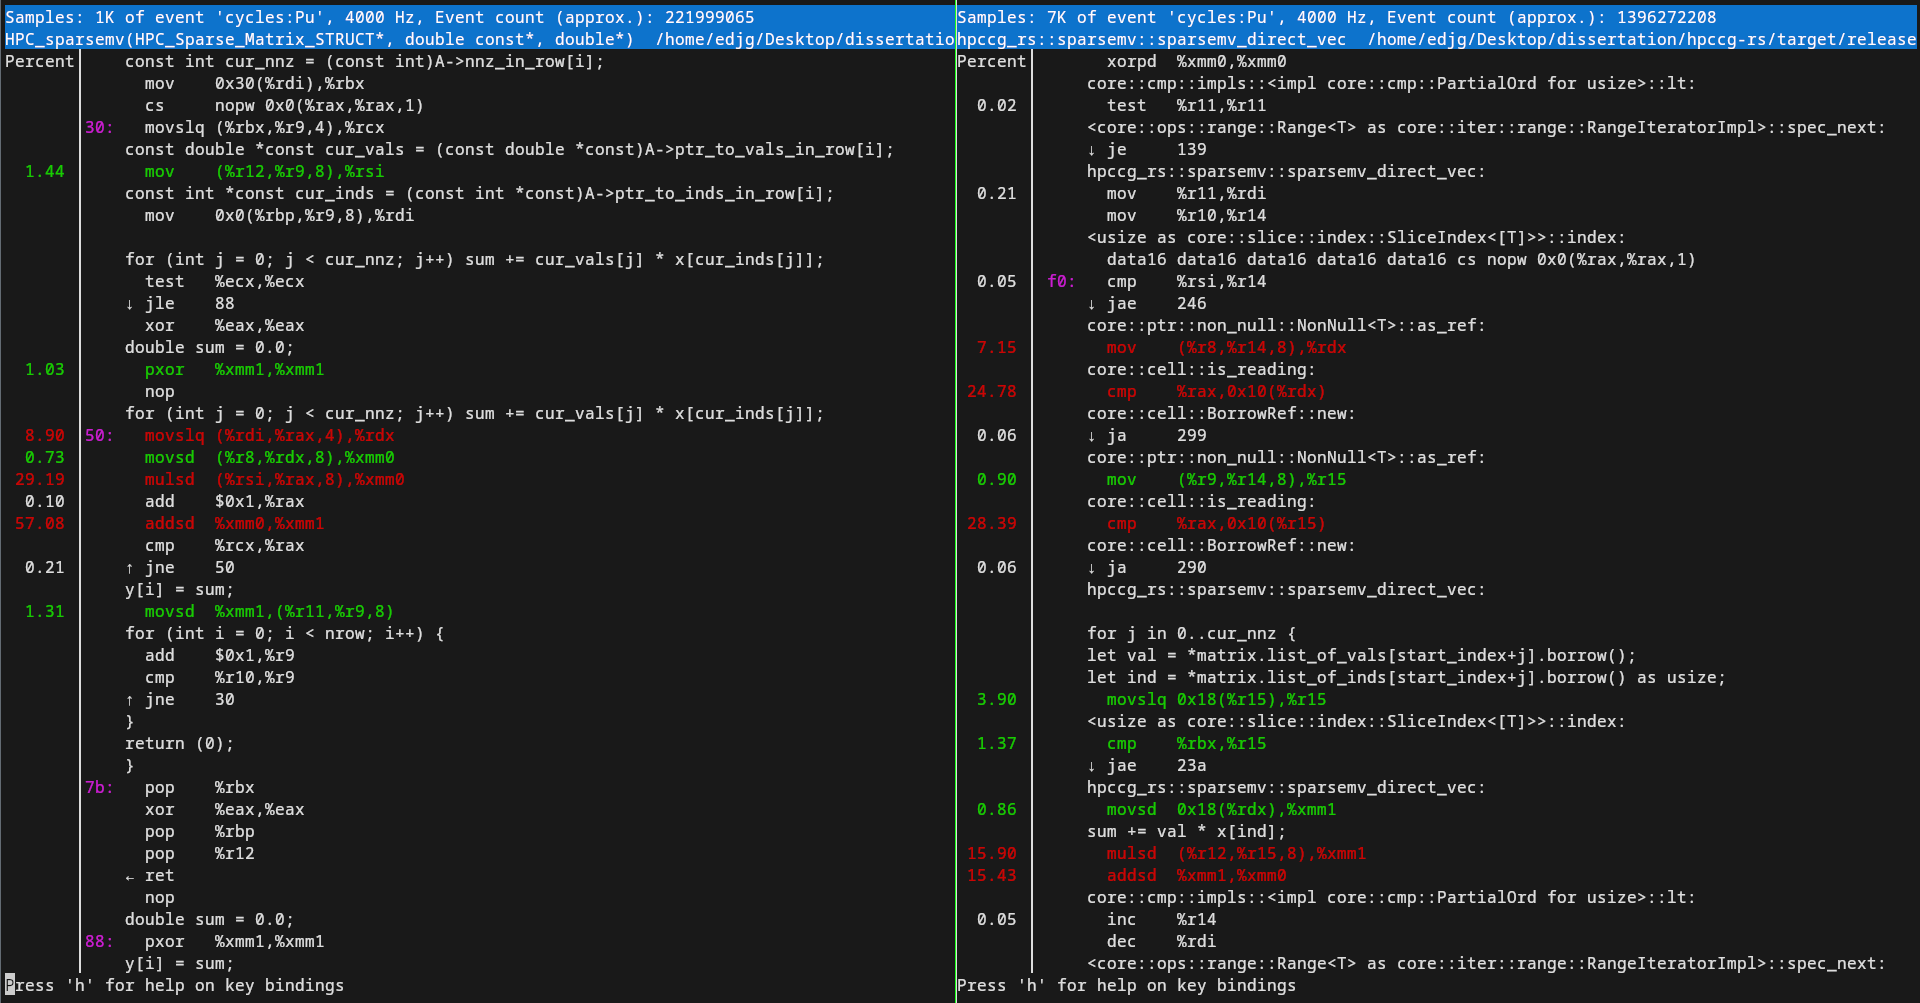
\includegraphics[width=0.85\textwidth]{images/perf_annot_cmp.png}
%         \caption{A screenshot of the \texttt{perf} tool showing hotspots in the C++ (left) and Rust (right) sparse matrix-vector multiplication kernels.}
%         \label{fig:perfAnnotCmp}
%     \end{figure}
% \end{frame}

% \begin{frame}{Analysis with \texttt{perf} \ ii}
%     \begin{figure}[H]
%         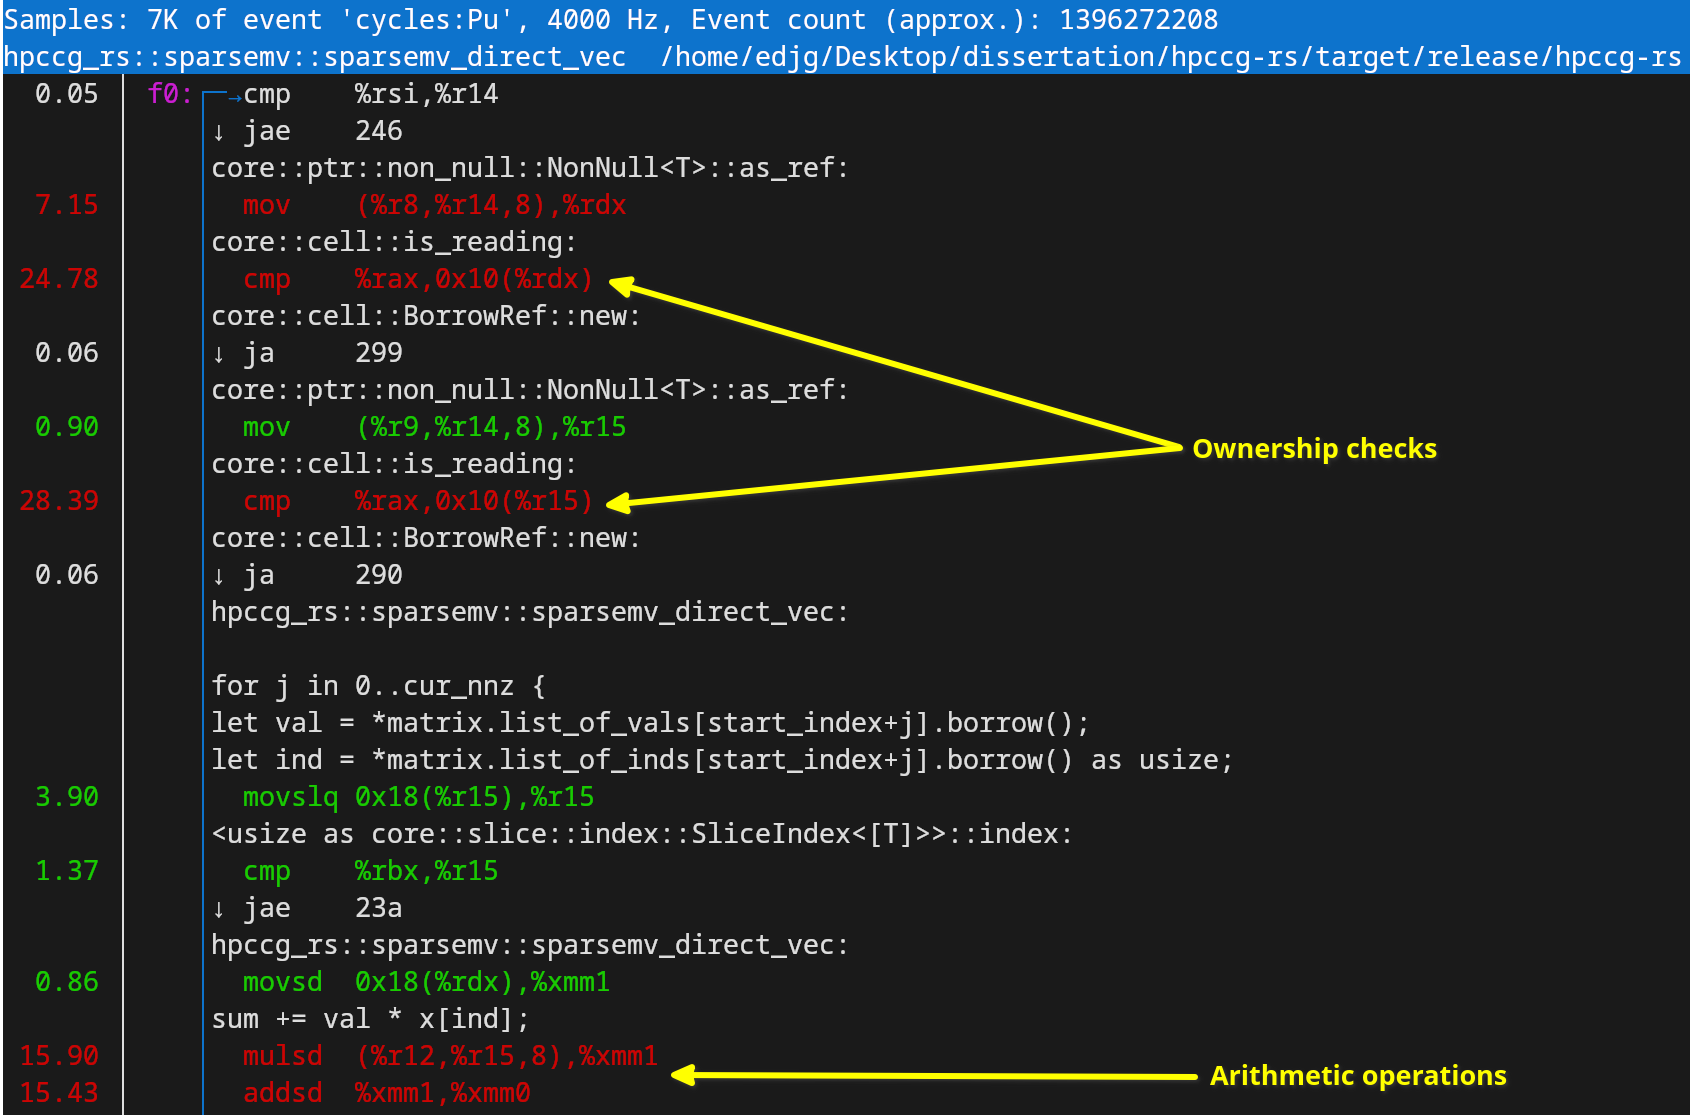
\includegraphics[width=0.65\textwidth]{images/perf_annot_labelled.png}
%         \caption{An annotated screenshot of the \texttt{perf} tool showing how ownership checks dominate the proportion of time taken in the Rust implementation, reducing total performance.}
%         \label{fig:perfAnnotLabelled}
%     \end{figure}
% \end{frame}

% \begin{frame}{Analysis with Intel\textsuperscript{\textregistered}\ vTune\texttrademark}
%     % TODO: Drop this slide
%     \begin{figure}[H]
%         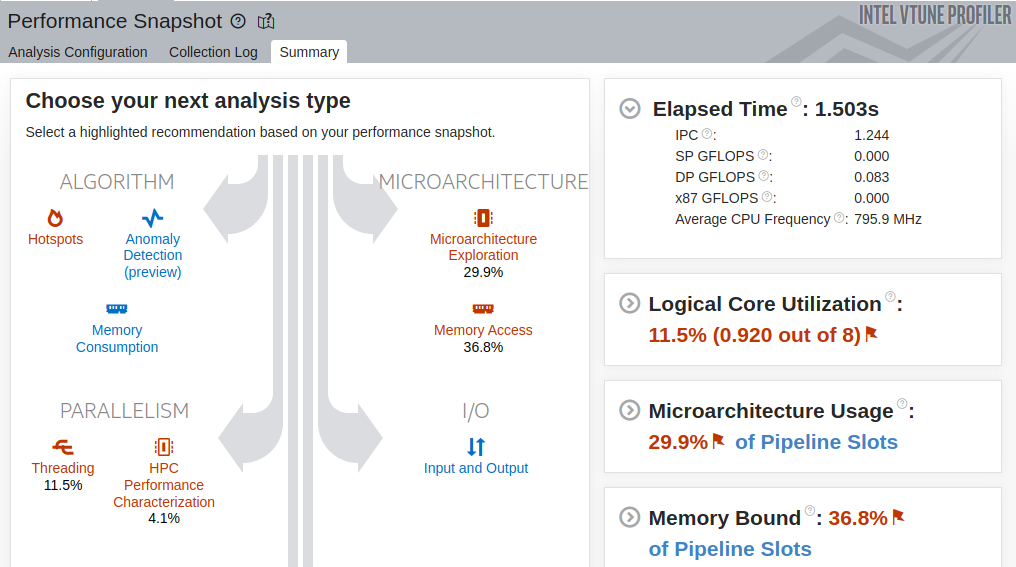
\includegraphics[width=0.85\textwidth]{images/intelvtune.png}
%         \caption{A screenshot of the summary page of Intel\textsuperscript{\textregistered}\ vTune\texttrademark\ when run on the Rust implementation.}
%         \label{fig:intelvtune}
%     \end{figure}
% \end{frame}

\begin{frame}{Novel tool \#2: HPC MultiBench \ i}
    \begin{itemize}
        \item<1-> Manually spawning many similar jobs with different configurations is tedious!
        \begin{itemize}
            \item Time consuming
            \item Susceptible to human error
            \item Discourages duplicating results for statistical confidence
        \end{itemize}
        \vspace{0.5cm}
        \item<2-> HPC MultiBench is a Python tool to define, run, and analyse batch compute jobs via Slurm from a convenient YAML format
    \end{itemize}
\end{frame}


\begin{frame}{Novel tool \#2: HPC MultiBench \ ii}
    \vspace{0.2cm}
    \large\begin{displayquote}
        ``Anything I have done in the past I think I could do in the YAML file.''\newline
        \hspace*{0.5cm}-- Toby Flynn (Warwick PhD candidate)
    \end{displayquote}
    \vspace{1cm}
    \large\begin{displayquote}
        ``I would use it for sure -- the problem you think exists definitely does.''\newline
        \hspace*{0.5cm} -- Sam Curtis (Warwick PhD candidate)
    \end{displayquote}
\end{frame}


\begin{frame}{Returning to the live demo}
    \note[item]{How a test plan can be defined using a YAML file}
    \note[item]{Automatic creation of runs specified by the YAML file}
    \note[item]{How metrics from completed runs can be aggregated and visualised}
    \note[item]{Directly measured results for comparing C++ and Rust performance}
    % By the end of this demo, I will have shown:
    % \begin{enumerate}
    %     \item How a test plan can be defined using a YAML file
    %     \item Automatic creation of runs specified by the YAML file
    %     \item How metrics from completed runs can be aggregated and visualised
    %     \item Directly measured results for comparing C++ and Rust performance
    % \end{enumerate}

    % TODO: Clickable link to backup slides
\end{frame}


% \begin{frame}{Overview of results \ i}
%     % Serial comparison
% \end{frame}
% \begin{frame}{Overview of results \ ii}
%     % Parallel comparison
% \end{frame}
% \begin{frame}{Overview of results \ iii}
%     % Multi-nodal MPI comparison
% \end{frame}
% \begin{frame}{Overview of results \ iv}
%     % Multi-nodal Hybrid comparison
% \end{frame}
% \begin{frame}{Overview of results \ v}
%     % CPP / Kokkos / Rust comparison
% \end{frame}
% \begin{frame}{Overview of results \ vi}
%     % Multi-nodal Strong scaling
% \end{frame}
% \begin{frame}{Overview of results \ vii}
%     % Multi-nodal Weak scaling
% \end{frame}
% \begin{frame}{Overview of results \ viii}
%     % Add `lscpu` for my machine alongside it
%     \begin{figure}[H]
%         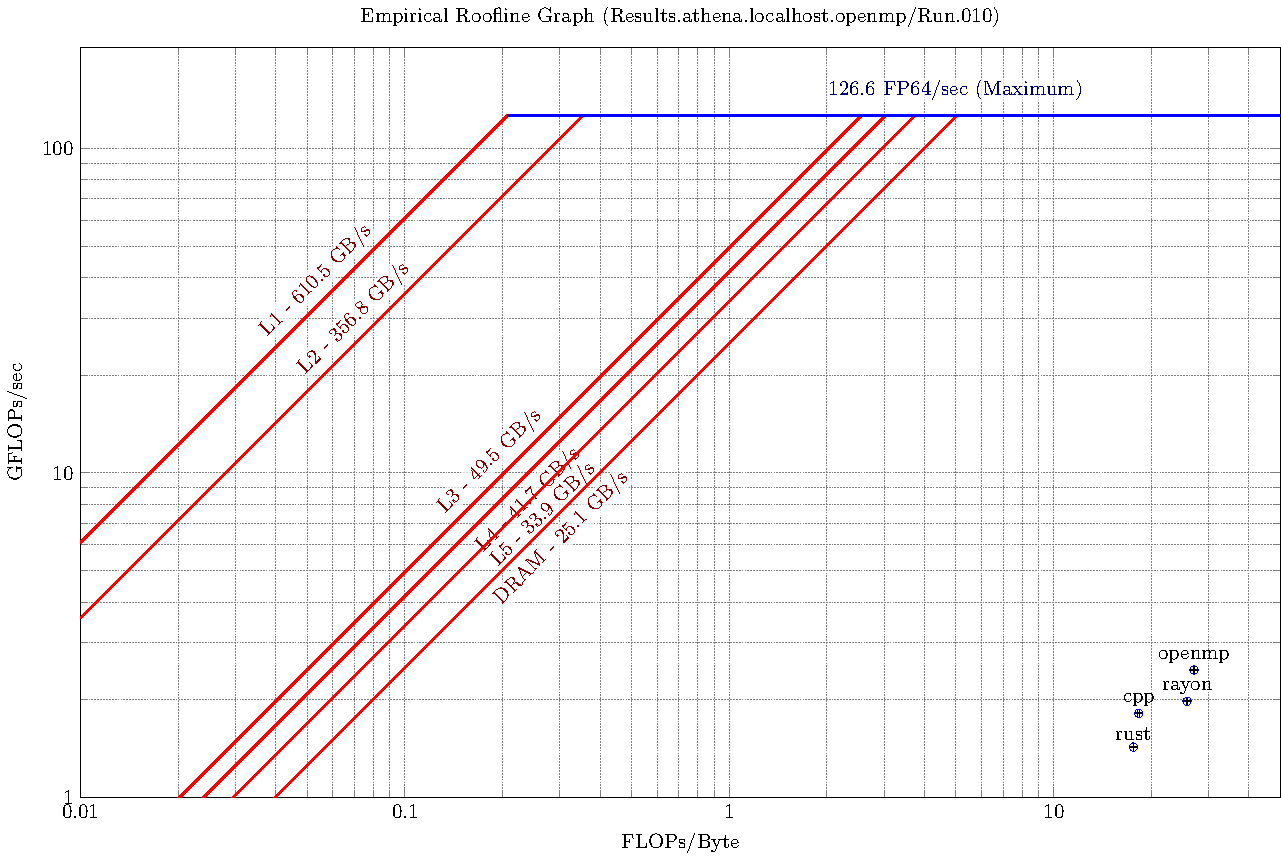
\includegraphics[width=0.65\textwidth]{images/Athena_ERT_generated_roofline.pdf}
%         \caption{A Roofline Diagram generated using the Empirical Roofline Toolkit \footcite{yangEmpiricalRooflineMethodology2018}, with data-points measured using LIKWID \footcite{treibigLIKWIDLightweightPerformance2012} showing serial and parallel implementations of HPCCG in Rust and C++.}
%         \label{fig:intelvtune}
%     \end{figure}
% \end{frame}
% \begin{frame}{Back to the plan...}
    % TODO: Clickable link back to here
% \end{frame}

\begin{frame}{Summary of Performance Analysis}
    % TODO: Add summary plot
    \begin{itemize}
        \item Rust is non-negligibly slower than C++
        \item In certain applications, this may be acceptable due to other commensurate benefits
    \end{itemize}
\end{frame}

\begin{frame}{Performance Analysis Requirements \ i}
    \begin{itemize}
        \item[\done\ 13.]
          Carry out a performance analysis of the serial translated Rust code with the original C++ code
          (\textbf{Must have}, \textit{depends on 5})
        \item[\done\ 14.]
          Carry out a performance analysis of the parallel translated Rust code with the original C++ code
          (\textbf{Must have}, \textit{depends on 11})
        \item[\done\ 17.]
          Carry out a performance analysis of the clustered translated Rust code with the original C++ code
          (\textbf{Could have}, \textit{depends on 15})
    \end{itemize}
\end{frame}






\section{Project management}

\begin{frame}{Agile Workflows}
    \begin{figure}[h]
        \centering
        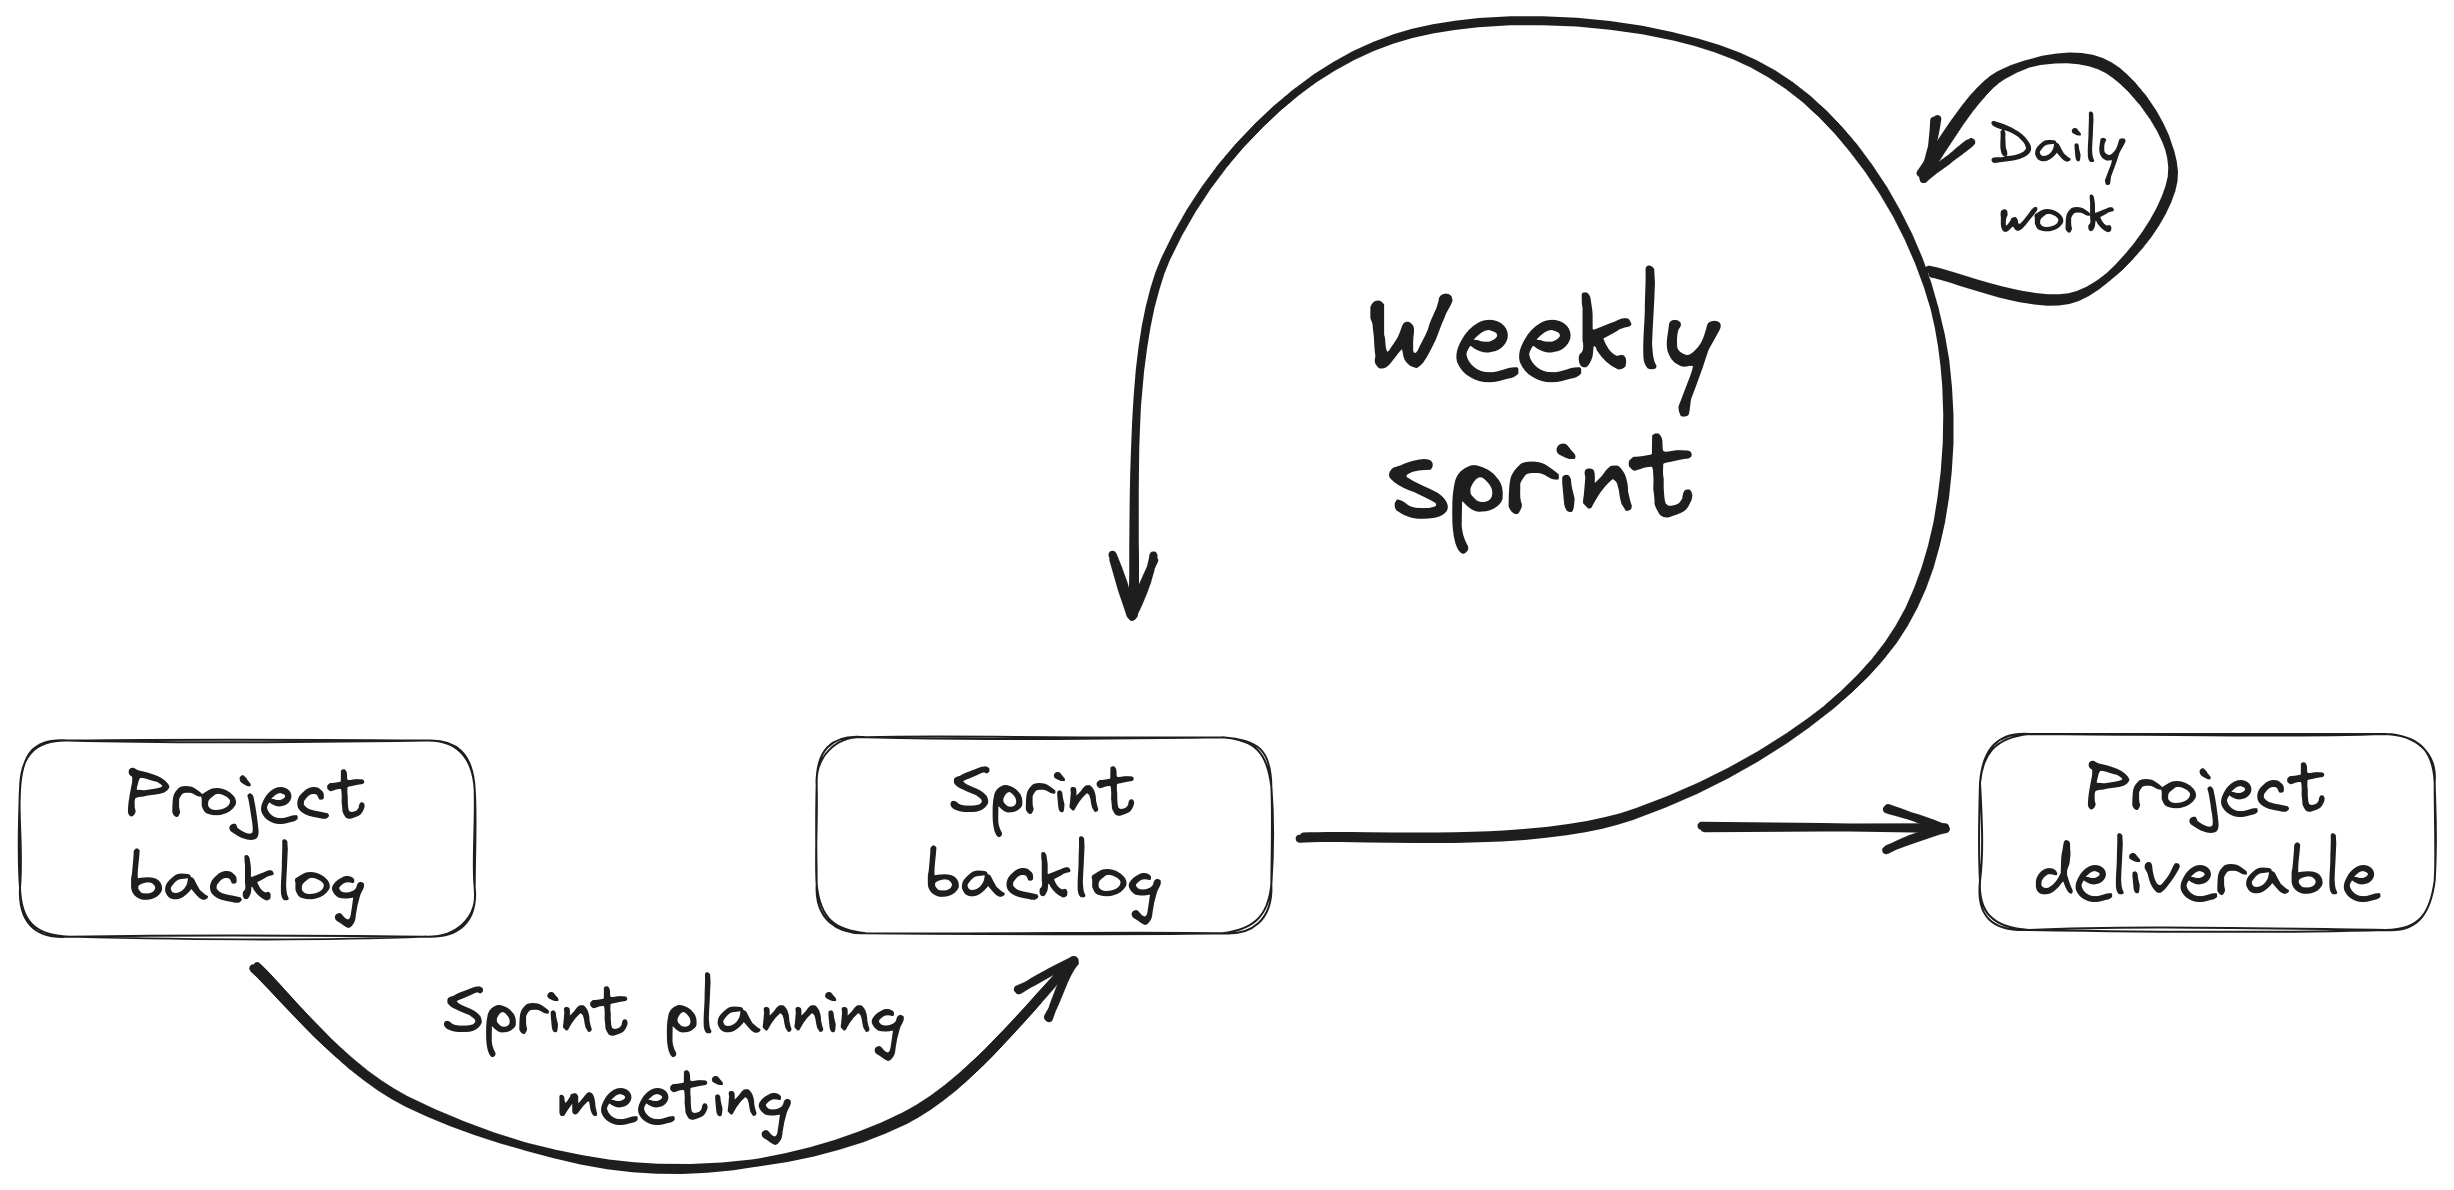
\includegraphics[width=0.6\textwidth]{images/excalidraw_agile.png}
        \caption{A diagram of a typical workflow for the Scrum flavour of Agile development.}
        \label{fig:specification_gantt_chart}
    \end{figure}

    \only<2->{
        \begin{tikzpicture}[remember picture,overlay]
            \node[xshift=-2.5cm,yshift=-1.75cm] at (current page.north east) {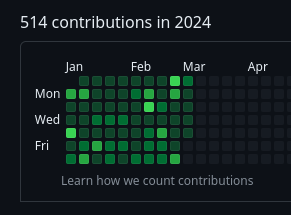
\includegraphics[width=0.25\textwidth]{images/github_commit_plot.png}};
        \end{tikzpicture}
        \begin{tikzpicture}[remember picture,overlay]
            \node[xshift=-1cm,yshift=-2.65cm] at (current page.north east) {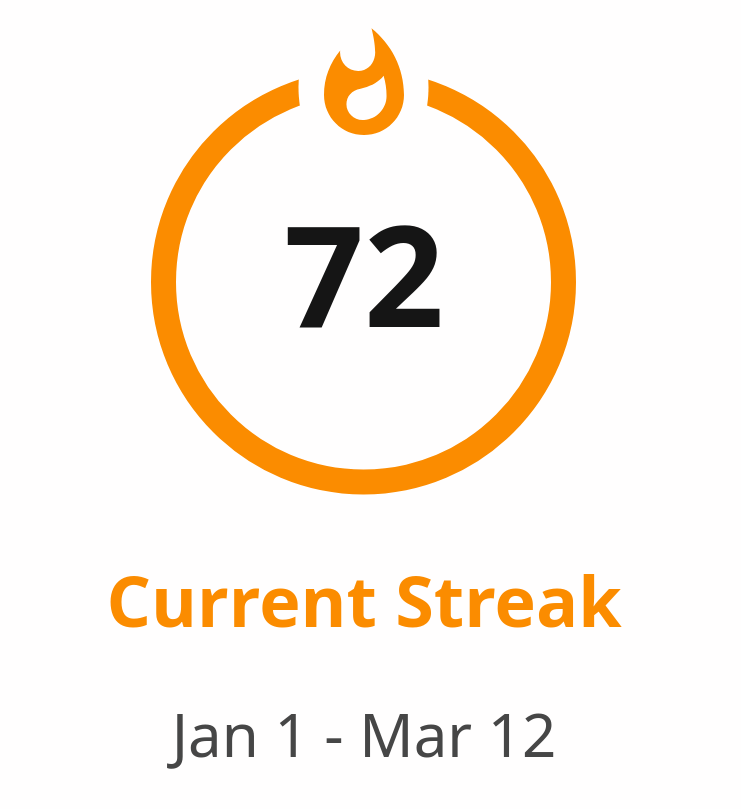
\includegraphics[width=0.115\textwidth]{images/github_streak.png}};
        \end{tikzpicture}
        \vspace*{-0.75cm}
    }

    \vspace*{-0.5cm}
    \begin{itemize}
        \item Weekly supervisor meetings, which bookend sprints
            \note[item]{Act as both sprint retrospective and planning}
            \note[item]{Agenda written up beforehand, then minutes submitted to Tabula afterwards\newline}
        \item Agile has empowered the project to be goal orientated and flexible to change \footcite{beckManifestoAgileSoftware2001}
            \note[item]{Goal orientation has allowed me to make a number of polished software products}
            \note[item]{Flexibility to change as allowed be to adapt the initial plan based on new information and ongoing supervisor discussion\newline}
        \item Daily work tracked in \texttt{git}
            \note[item]{By daily - I really mean daily! Continuous streak of $\geq 1$ commit every day this year}
    \end{itemize}
    \vspace*{0.5cm}
\end{frame}

\begin{frame}{Specification Timeline}
    \begin{figure}[h]
        \centering
        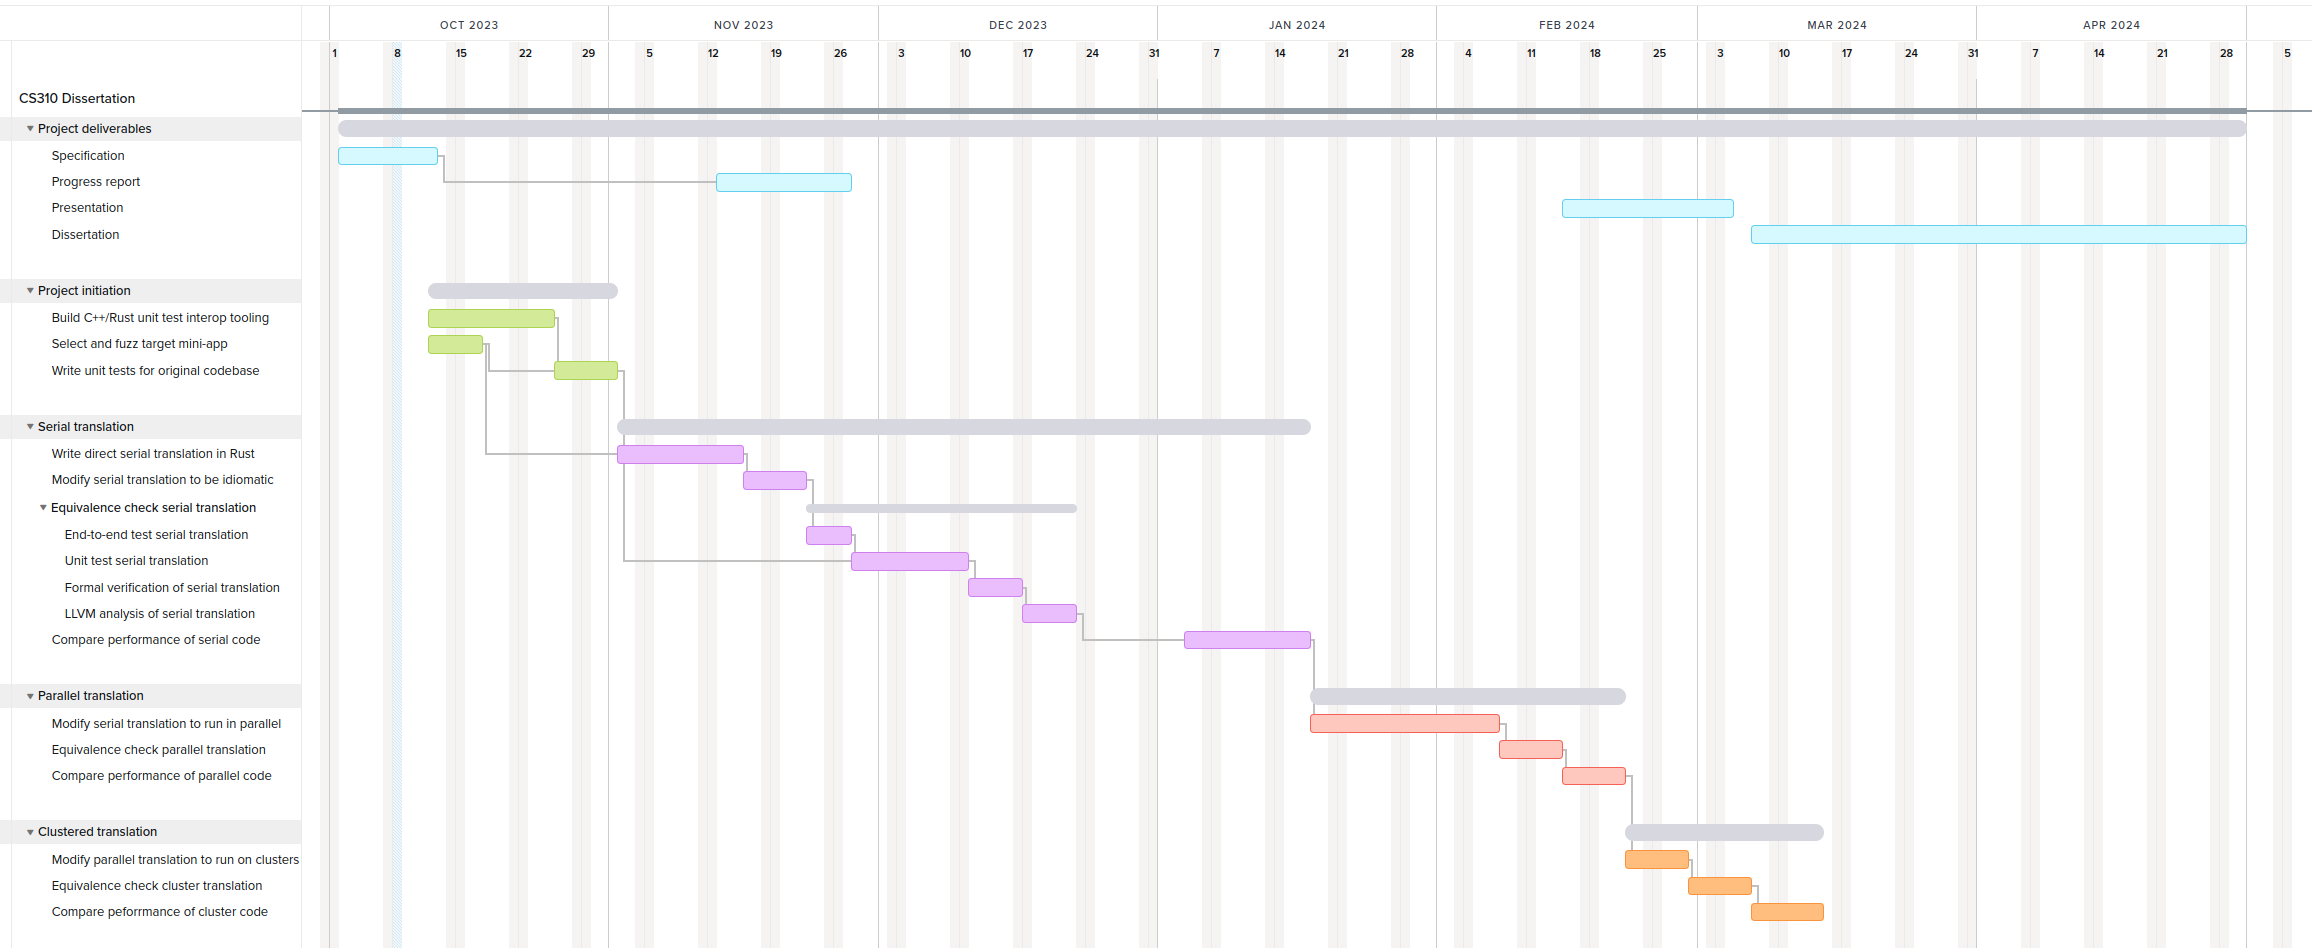
\includegraphics[width=\textwidth]{images/specification_gantt_chart.png}
        \caption{The original timeline from my specification}
        \label{fig:specification_gantt_chart}
    \end{figure}
\end{frame}

\begin{frame}{Actual Timeline}
    % Consider merging with previous slide
    \begin{figure}[h]
        \centering
        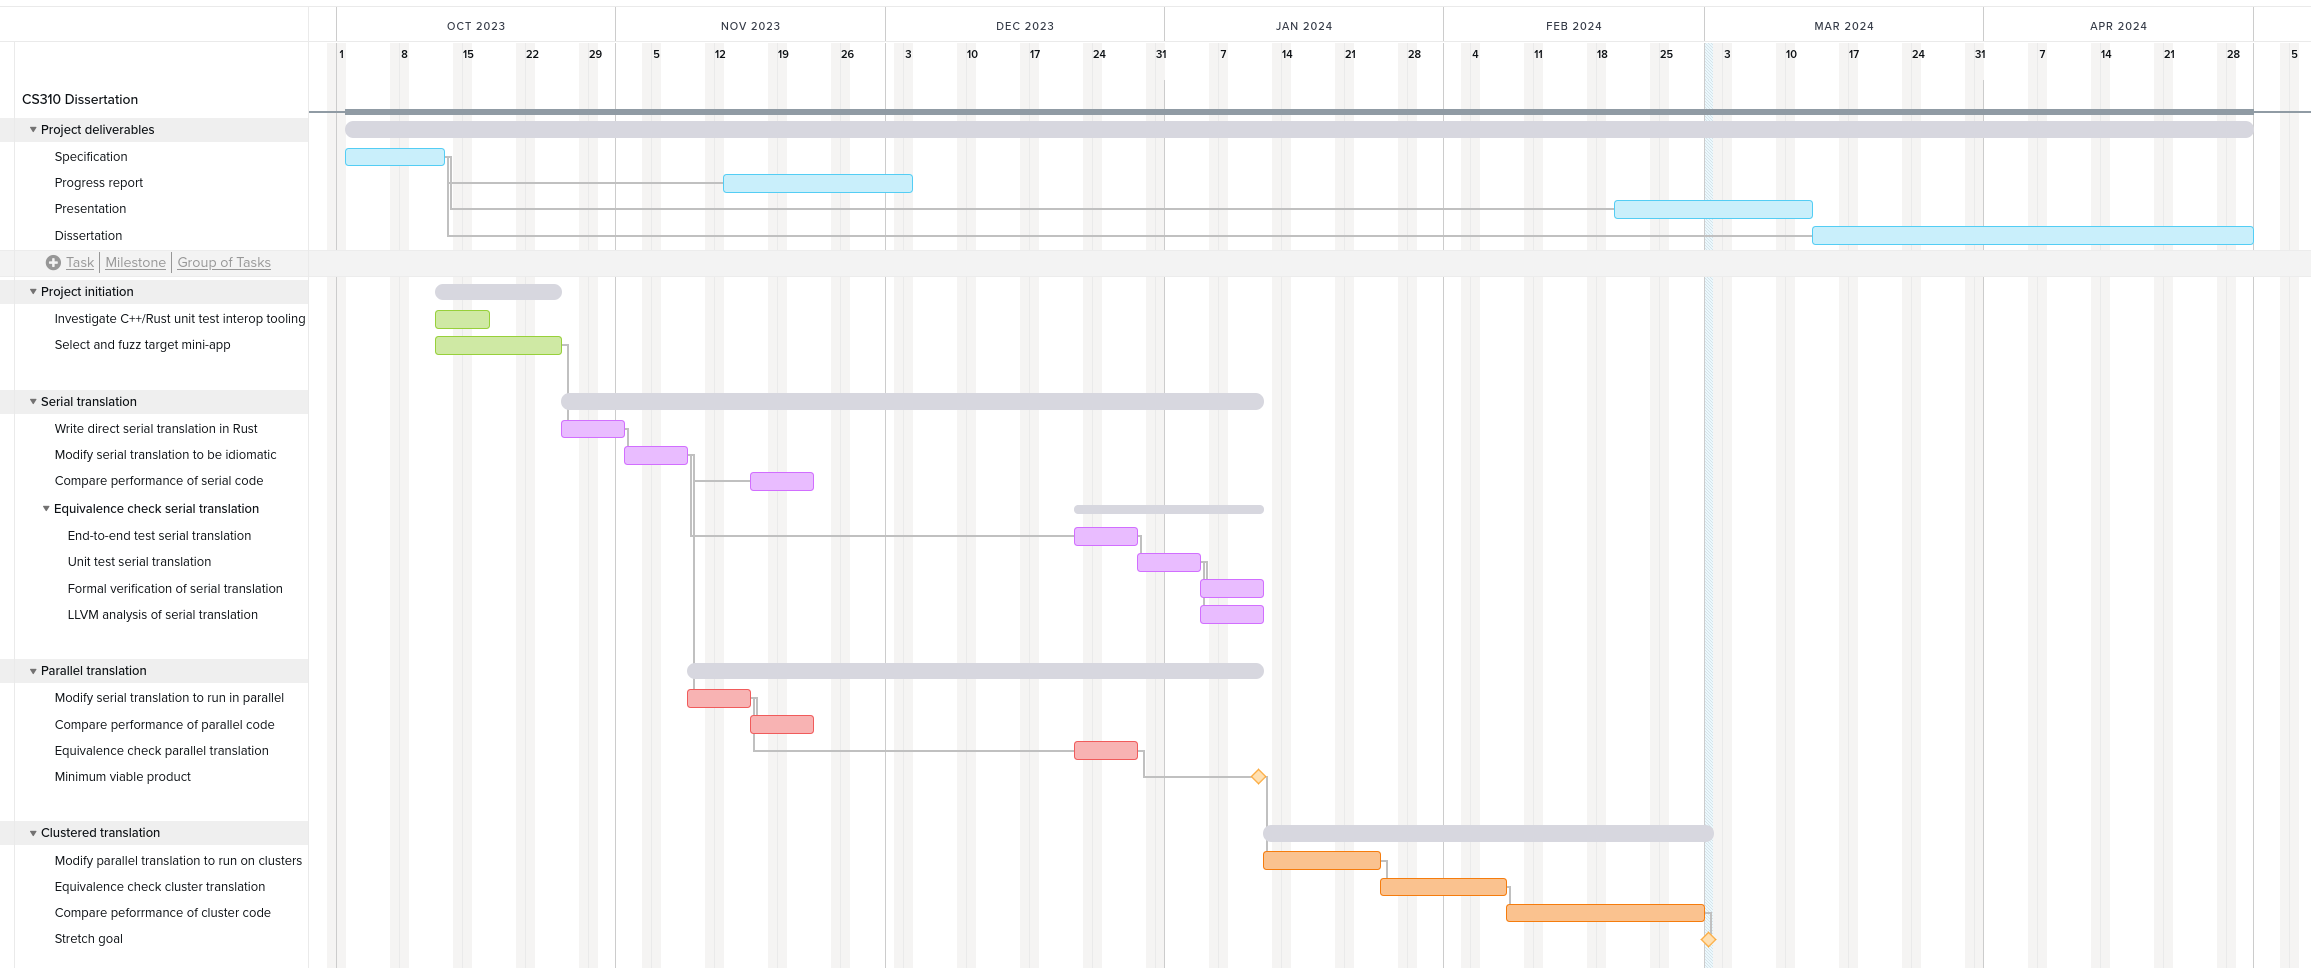
\includegraphics[width=\textwidth]{images/actual_gantt_chart.png}
        \caption{The actual timeline of the project. The progress report was more all-encompassing, parallelisation was easier, and clustering was harder than expected}
        % \caption{The actual timeline of the project. An agile methodology allowed me to overcome the fact that the progress report was more all-encompassing, parallelisation was easier, and clustering was harder than expected}
        \label{fig:actual_gantt_chart}
    \end{figure}
\end{frame}

% \begin{frame}{Unforeseen problems}
% \end{frame}


\section{Conclusion}

% \begin{frame}{Requirements \ i}
%     \begin{itemize}
%         \item[\done\ \ 1.]
%           Select a target mini-app from ECP proxy applications or UK-MAC
%           (\textbf{Must have})
%         \item[\done\ \ 2.]
%           Fuzz test\footnote{an automated testing technique which uses boundary and erroneous test data as inputs, whilst monitoring for resultant undesired behaviour, originally proposed by Miller \textit{et al.} in 1990 \footcite{millerEmpiricalStudyReliability1990}\footcite{liangFuzzingStateArt2018}} the possible mini-apps for memory safety issues using static analysis tooling \footcite{stepanovMemorySanitizerFastDetector2015}
%           (\textbf{Should have}, \textit{depends on 1})
%         \item[\done\ \ 3.]
%           Build tooling for running Rust unit tests on C++ code
%           (\textbf{Could have})
%         \item[\done\ \ 4.]
%           Write unit tests for the original C++ version of the
%           mini-app
%           (\textbf{Should have}, \textit{depends on 1, (3)})
%         \item[\done\ \ 5.]
%           Write direct translation of serial version mini-app from C++ to Rust
%           (\textbf{Must have}, \textit{depends on 1})
%         \item[\done\ \ 6.]
%           Modify serial version of translated code to be idiomatic Rust \footcite{endlerMreIdiomaticrust2023} 
%           (\textbf{Should have}, \textit{depends on 5})
%     \end{itemize}
% \end{frame}

% \begin{frame}{Requirements \ ii}
%     \begin{itemize}
%         \item[\done\ \ 7.]
%           Equivalence check serial translated code by comparing results of end-to-end tests with original C++ code
%           (\textbf{Must have}, \textit{depends on 5}))
%         \item[\done\ \ 8.]
%           Equivalence check serial translated code by applying passing C++ unit tests to rust code
%           (\textbf{Must have}, \textit{depends on 4, 5})
%         \item[\wontfix\ \ 9.]
%           Equivalence check serial translated code with limited formal verification techniques
%           (\textbf{Could have}, \textit{depends on 5})
%         \item[\partialdone\ 10.]
%           Equivalence check serial translated code by comparing generated LLVM IR of the C++ and translated Rust versions
%           (\textbf{Could have}, \textit{depends on 5})
%         \item[\done\ 11.]
%           Modify the serial translated code to allow parallel execution
%           (\textbf{Must have}, \textit{depends on 5})
%         \item[\done\ 12.]
%           Equivalence check parallel translated code via all previous techniques
%           (\textbf{Must have}, \textit{depends on 7, 8, (9), (10), 11})
%         \item[\done\ 13.]
%           Carry out a performance analysis of the serial translated Rust code with the original C++ code
%           (\textbf{Must have}, \textit{depends on 5})
%     \end{itemize}
% \end{frame}

% \begin{frame}{Requirements \ iii}
%     \begin{itemize}
%         \item[\done\ 14.]
%           Carry out a performance analysis of the parallel translated Rust code with the original C++ code
%           (\textbf{Must have}, \textit{depends on 11})
%         \item[\done\ 15.]
%           Modify the parallel translated code to allow execution across clustered compute resources
%           (\textbf{Could have}, \textit{depends on 11})
%         \item[\done\ 16.]
%           Equivalence check clustered translated code via all previous techniques
%           (\textbf{Could have}, \textit{depends on 7, 8, (9), (10), 15})
%         \item[\done\ 17.]
%           Carry out a performance analysis of the clustered translated Rust code with the original C++ code
%           (\textbf{Could have}, \textit{depends on 15})
%     \end{itemize}
% \end{frame}

\begin{frame}{Evaluation}
    \begin{itemize}
        \item Achieved all \textbf{M}ust/\textbf{S}hould have specification points, including stretch goal of assessing clustered compute
        \item ``Assessed the Viability of Rust in HPC'', answering the project question
        \vspace{0.5cm}
        \item<2-> \alert{Actively improved} the viability of Rust in HPC, by:
        \begin{itemize}
            \item Developing tools and workflows to assist in translation efforts
            \item Making open source contributions of tests and documentation
        \end{itemize}
    \end{itemize}
\end{frame}


\begin{frame}{Open Source Work}
    \begin{itemize}
        \item Pull requests to existing projects
        \begin{itemize}
            \item Integration tests for array operations to \texttt{autocxx}
            \item Plan to pull request documentation to both \texttt{autocxx} and \texttt{rs-mpi}
            % kokkos mini-apps add HPCCG Kokkos version
        \end{itemize}
        \vspace*{0.25cm}
        \item Repositories to release once project has been assessed
        \begin{itemize}
            \item \texttt{hpccg-rs} A Rust translation of the HPCCG mini-application
            \item \texttt{hpccg-kokkos} A Kokkos translation of the HPCCG mini-application
            \item \texttt{polyglotest} A mini-framework for pure test-driven development of Rust code translated from C++
            \item \texttt{HPC\_MultiBench} A tool to spawn and analyse Slurm jobs for performance benchmarking
        \end{itemize}
    \end{itemize}
\end{frame}

\begin{frame}{Future work}
\begin{itemize}
    \item<1-> Further research points if the project were longer:
    \begin{itemize}
        \item Translate a second, larger, mini-app such as MiniMD \footcite{osti_1231191} or HPCG \footcite{dongarra2015hpcg}
        \item Extend comparisons to include Rust GPU support
        % Better kokkos comparison
    \end{itemize}
    \vspace{1cm}
    \item<2-> \alert{Publish and maintain novel tools developed} as open source repositories
    \begin{itemize}
        \item If any of them start getting interest, will respond to pull requests/issues as far as possible
    \end{itemize}
    \item<3-> \alert{Aim to submit a paper} based on the project to P3HPC
\end{itemize}
\end{frame}




\appendix

% \begin{frame}[allowframebreaks]{References}
%   % \nocite{*}
%   \bibliographystyle{IEEEtran}
%   \bibliography{references}
% \end{frame}

\begin{frame}[allowframebreaks]{Bibliography}
    \printbibliography[heading=none]
\end{frame}

\section{Backup Slides}

\begin{frame}{Backup Slides \ i}
\end{frame}

% \begin{frame}[fragile]{Typography}
%       \begin{verbatim}The theme provides sensible defaults to
% \emph{emphasize} text, \alert{accent} parts
% or show \textbf{bold} results.\end{verbatim}

%   \begin{center}becomes\end{center}

%   The theme provides sensible defaults to \emph{emphasize} text,
%   \alert{accent} parts or show \textbf{bold} results.
% \end{frame}

% \begin{frame}{Font feature test}
%   \begin{itemize}
%     \item Regular
%     \item \textit{Italic}
%     \item \textsc{SmallCaps}
%     \item \textbf{Bold}
%     \item \textbf{\textit{Bold Italic}}
%     \item \textbf{\textsc{Bold SmallCaps}}
%     \item \texttt{Monospace}
%     \item \texttt{\textit{Monospace Italic}}
%     \item \texttt{\textbf{Monospace Bold}}
%     \item \texttt{\textbf{\textit{Monospace Bold Italic}}}
%   \end{itemize}
% \end{frame}

% \begin{frame}{Multiple images on one slide}
% \begin{figure}
%     \begin{overprint}
%     \onslide<1>\includegraphics{./figure1.png}
%     \onslide<2>\includegraphics{./figure2.png}
%     \onslide<3>\includegraphics{./figure3.png}
%     \onslide<4->\includegraphics{./figure4.png}
%     \end{overprint}
% \end{figure}
% \end{frame}

% \begin{frame}{Columns}
%   \begin{columns}[T,onlytextwidth]
%     \column{0.5\textwidth}
%       Items
%       \begin{itemize}
%         \item Milk \item Eggs \item Potatos
%       \end{itemize}

%     \column{0.5\textwidth}
%       Enumerations
%       \begin{enumerate}
%         \item First, \item Second and \item Last.
%       \end{enumerate}
%   \end{columns}
% \end{frame}

% \begin{frame}{Animation}
%   \begin{itemize}[<+- | alert@+>]
%     \item \alert<4>{This is\only<4>{ really} important}
%     \item Now this
%     \item And now this
%   \end{itemize}
% \end{frame}

% \begin{frame}{Figures}
%   \begin{figure}
%     \newcounter{density}
%     \setcounter{density}{20}
%     \begin{tikzpicture}
%       \def\couleur{alerted text.fg}
%       \path[coordinate] (0,0)  coordinate(A)
%                   ++( 90:5cm) coordinate(B)
%                   ++(0:5cm) coordinate(C)
%                   ++(-90:5cm) coordinate(D);
%       \draw[fill=\couleur!\thedensity] (A) -- (B) -- (C) --(D) -- cycle;
%       \foreach \x in {1,...,40}{%
%           \pgfmathsetcounter{density}{\thedensity+20}
%           \setcounter{density}{\thedensity}
%           \path[coordinate] coordinate(X) at (A){};
%           \path[coordinate] (A) -- (B) coordinate[pos=.10](A)
%                               -- (C) coordinate[pos=.10](B)
%                               -- (D) coordinate[pos=.10](C)
%                               -- (X) coordinate[pos=.10](D);
%           \draw[fill=\couleur!\thedensity] (A)--(B)--(C)-- (D) -- cycle;
%       }
%     \end{tikzpicture}
%     \caption{Rotated square from
%     \href{http://www.texample.net/tikz/examples/rotated-polygons/}{texample.net}.}
%   \end{figure}
% \end{frame}

% \begin{frame}{Tables}
%   \begin{table}
%     \caption{Largest cities in the world (source: Wikipedia)}
%     \begin{tabular}{lr}
%       \toprule
%       City & Population\\
%       \midrule
%       Mexico City & 20,116,842\\
%       Shanghai & 19,210,000\\
%       Peking & 15,796,450\\
%       Istanbul & 14,160,467\\
%       \bottomrule
%     \end{tabular}
%   \end{table}
% \end{frame}

% \begin{frame}{Blocks}
%   Three different block environments are pre-defined and may be styled with an optional background color.
  
%   \metroset{block=fill}
%   \begin{block}{Default}
%     Block content.
%   \end{block}
%   \begin{alertblock}{Alert}
%     Block content.
%   \end{alertblock}
%   \begin{exampleblock}{Example}
%     Block content.
%   \end{exampleblock}
% \end{frame}

% \begin{frame}{Math}
%   \begin{equation*}
%     e = \lim_{n\to \infty} \left(1 + \frac{1}{n}\right)^n
%   \end{equation*}
% \end{frame}

% \begin{frame}{Line plots}
%   \begin{figure}
%     \begin{tikzpicture}
%       \begin{axis}[
%         mlineplot,
%         width=0.9\textwidth,
%         height=6cm,
%       ]

%         \addplot {sin(deg(x))};
%         \addplot+[samples=100] {sin(deg(2*x))};

%       \end{axis}
%     \end{tikzpicture}
%   \end{figure}
% \end{frame}

% \begin{frame}{Bar charts}
%   \begin{figure}
%     \begin{tikzpicture}
%       \begin{axis}[
%         mbarplot,
%         xlabel={Foo},
%         ylabel={Bar},
%         width=0.9\textwidth,
%         height=6cm,
%       ]

%       \addplot plot coordinates {(1, 20) (2, 25) (3, 22.4) (4, 12.4)};
%       \addplot plot coordinates {(1, 18) (2, 24) (3, 23.5) (4, 13.2)};
%       \addplot plot coordinates {(1, 10) (2, 19) (3, 25) (4, 15.2)};

%       \legend{lorem, ipsum, dolor}

%       \end{axis}
%     \end{tikzpicture}
%   \end{figure}
% \end{frame}

% \begin{frame}[fragile]{Code Snippets}
%     Code snippets with syntax highlighting can be embedded using then \verb|minted| package:
%     \begin{minted}[escapeinside=||]{haskell}
% newtype Lasagne = Lasagne Int
%     deriving (Show, Num)

% -- The stacking operating can be considered integer 
% -- addition of the number of layers
% instance Semigroup Lasagne where
%     (<>) = (+)
%     \end{minted}
% \end{frame}


\end{document}
